% allows for alternative text
% \DocumentMetadata{
%     tagging=on,
%     tagging-setup={math/setup=mathml-SE},
%     pdfstandard=ua-2,
%     lang=en-US
% }

\documentclass{tstextbook}

%---------------------------------------------------------------------------
% Added packages
%---------------------------------------------------------------------------
\usepackage{wrapfig}
\usepackage{framed}
\usepackage{soul}
\usepackage[dvipsnames]{xcolor}
\usepackage{mdframed}
\usepackage{comment}
\usepackage{mathrsfs}
\usepackage{enumitem}
\usepackage{physics}
\usepackage{amsmath}
\usepackage{listings}
\usepackage{graphicx}


\renewcommand{\thefootnote}{\fnsymbol{footnote}}

% ----- MATLAB listing environment ----- from Nils
\usepackage[T1]{fontenc}
\usepackage{inconsolata}
% \usepackage[numbered,framed]{matlab-prettifier}
\definecolor{codegreen}{rgb}{0,0.6,0}
\definecolor{codegray}{rgb}{0.5,0.5,0.5}
\definecolor{codepurple}{rgb}{0.58,0,0.82}
\lstdefinestyle{mystyle}{
    backgroundcolor=\color{white},
    commentstyle=\color{codegreen},
    keywordstyle=\color{magenta},
    stringstyle=\color{codepurple},
    basicstyle=\ttfamily\footnotesize,
    breakatwhitespace=false,
    breaklines=true,
    captionpos=b,
    keepspaces=true,
    numbers=none,
    showspaces=false,
    showstringspaces=false,
    showtabs=false,
    tabsize=2,
    frame=none
}
\lstset{style=mystyle}

\setlength{\arrayrulewidth}{0.4mm}
\setlength{\tabcolsep}{10pt}
\renewcommand{\arraystretch}{1.5}

\setcounter{MaxMatrixCols}{20}


\newcommand{\quo}[1]{``#1"}

\usepackage{amsthm}
\theoremstyle{remark}
\newmdtheoremenv[
    linewidth=0.4mm,
    linecolor=tsorange2,
    backgroundcolor=tsorange2!8,
    skipabove=6pt,
    skipbelow=6pt,
    innertopmargin=6pt,
    innerbottommargin=6pt
]{remark}{Remark}

%---------------------------------------------------------------------------
% Textbook contents
%---------------------------------------------------------------------------
\makeindex

\begin{document}



\tsbook{Numerical Solutions to \\ Partial Differential Equations}   % Textbook name
       {| Brennan Sprinkle and Rachel Bertaud |} % Author(s)
       {Rachel Bertaud}                                    % Cover Artist
       {2026}                                               % Publication year



%---------------------------------------------------------------------------
% Chapters
%---------------------------------------------------------------------------


\chapter{How to Visually Communicate}
\label{chpt:visComm}


 Pictures, figures, images, plots, etc. are all forms of visual communication. Any visual communication should be made in the most \textit{effective} and \textit{accessible} way possible. This chapter will discuss what it means to visually communicate effectively and ensure accessibility when creating line and field plots from data. General implementation of these practices in python and MATLAB is provided in Section~\ref{chpt:figCode}. 

\index{plotting}
\index{figure making}

\section{Effective and Accessible Communication}
\label{chpt:effectiveFigs}
Visual communication is effective when the reader immediately understands what is being presented. Labels, such as those in legends and on axes, tell the reader exactly what is presented without the need for assumptions or guessing. Units for the axes set scale which allows the reader to form conclusions of their own without further explanation. Captions describe the visualization in words and include what the reader needs to understand the plot's labels, such as variable definitions. Note that conclusions or analysis \textit{should not} be discussed in captions. Plots can imply if the data is discrete or continuous by using data symbols (scatter plots) or continuous curves (solid lines). Data are generally discrete and should be plotted using symbols, while theory/fits should be plotted as continuous curves. All of these stylistic choices discussed make visual communication more effective.

For visual communication to be completely accessible, no reader should be at a disadvantage due to physical abilities or technological access. Colorblindness can make data difficult to discern if the colors do not contrast, especially when considering those who are completely colorblind or when work is printed in black and white. Efforts to use more than color, such as markers, and to select contrasting colors ensure general readability no matter the case. Assistive technology is capable of converting visual communication to non-visual communication by reading alternative text of images. When publicizing work, it is important to include and use descriptive alternative text so that any visual communication can be understood without seeing the image or figure. 

The next two subsections will discuss class standards for visual communication for line and field plots. Code used to produce plots seen in Figures~\ref{fig:badLines!} and \ref{fig:exampField} is provided in Section~\ref{chpt:figCode}.

\newpage
\subsection{Line Plots}
Consider the presentation of data in Figure~\ref{fig:badLines!}. The figure is arranged in two columns: column (1), on the left, shows a poorly made plot, while column (2), on the right, shows a well-constructed one. The three rows \emph{(a)}, \emph{(b)}, and \emph{(c)} correspond to full RGB color, color as experienced with protanopia (red–green colorblindness), and grayscale, respectively. Table~\ref{tab:lineComparison} compares each flaw of plot (1) with its correction in column (2).


\begin{table}[h!]
    \centering
    \begin{tabular}{|>{\raggedright\arraybackslash}p{3cm}|>{\raggedright\arraybackslash}p{4cm}||>{\raggedright\arraybackslash}p{6cm}|}
        \hline
        \textit{Bad plot traits (seen in 1)} & \textit{Good plot traits \ \ \ \ \ \ \ \  (seen in 2)} & \textit{Impact to reader} \\
        \hline
        No data symbols & Large, differentiable data symbols & Shows where the data actually is. \textbf{Symbols represent data; curves represent theory/fits.} {\small Symbols also keep data distinguishable in the legend and plot when color fails (e.g., poor projector or paper printout).} \\
        Small tick labels (numbers on axes) & Large labels everywhere & \textbf{Make everything larger than you think!} Easier for the viewer to read and interpret the data. \\
        No labels for data, plot, or axes & Fully labeled plot \textbf{with units} & Tells the reader what is being presented and the scale of the problem. \\
        Similar colors for different data & Unique, contrasting colors for each dataset & Keeps data distinguishable for colorblind readers and in grayscale, shown in plots (b) and (c). Similar RGB colors can become identical in both cases. \\
        Linearly scaled axes & Logarithmically scaled axes & Reveals power-law behavior. \\
        No reference lines & Reference lines for $n$-order convergence & Confirms to the reader that the claimed order of convergence is actually achieved. \\
        Programs default font (mismatched with document) & Font matching the document body (e.g., Latin Modern) & Makes plot text consistent with the surrounding \LaTeX{} type, so figures don't look pasted in. \textbf{Computer/Latin Modern or Helvetica/Free Sans are strongly recommended.} \\
        \hline
    \end{tabular}
    \caption{Description of differences in plots shown in Figure~\ref{fig:badLines!} and their impact on readability.}
    \label{tab:lineComparison}
\end{table}


\begin{figure}[!ht]
\begin{framed}
  % ---- Row 1 ----
  \emph{1}(\emph{a})
  \hspace*{7cm}
  \emph{2}(\emph{a})\\
  \hspace*{5mm}
  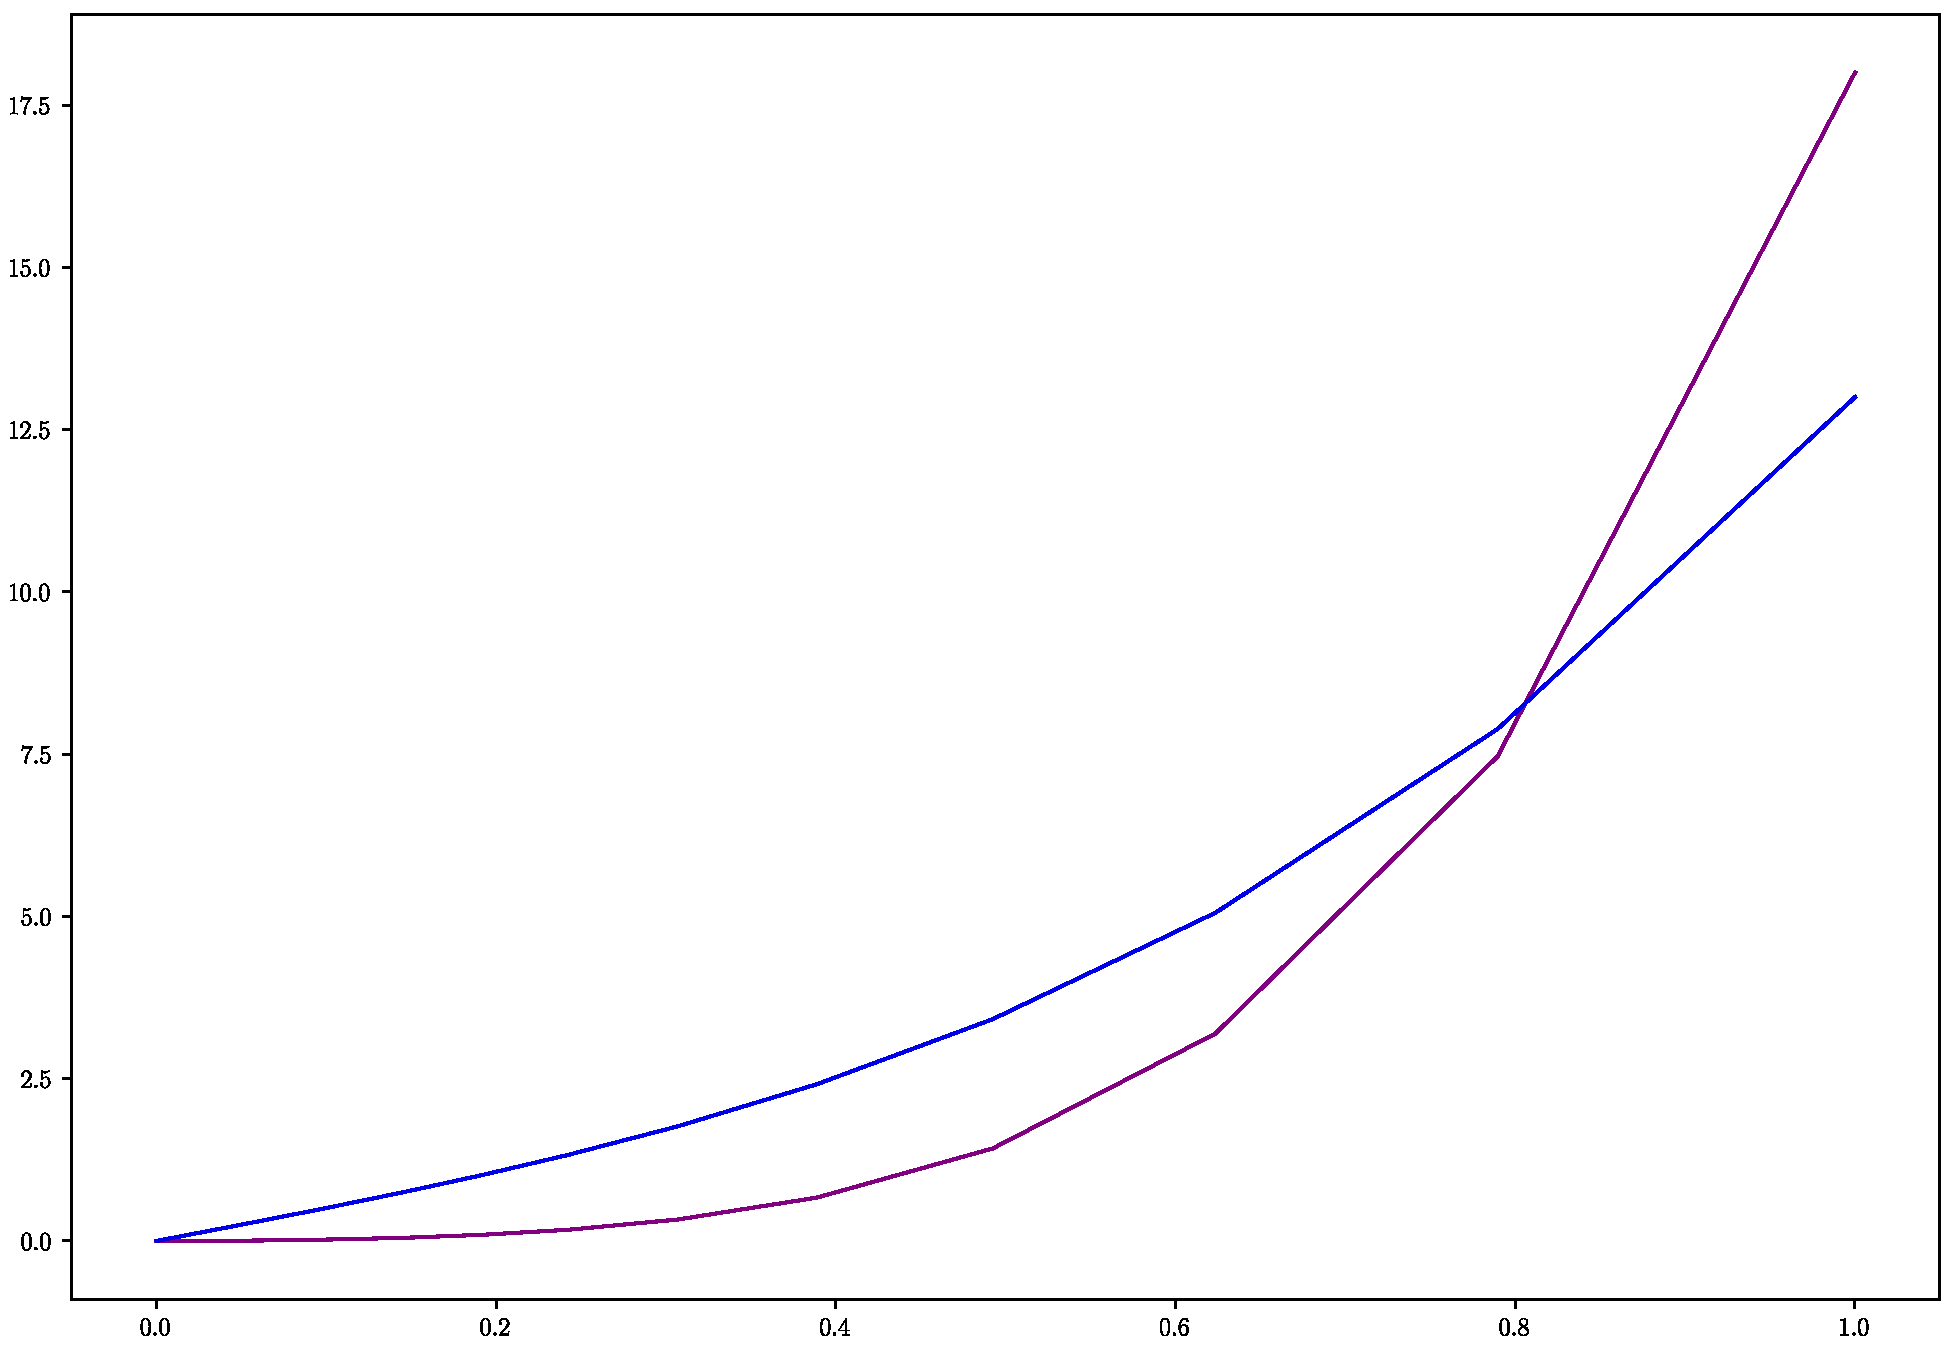
\includegraphics[trim = 0mm 0mm 0mm 0mm,clip,
  width=7.0cm, page=1]{Plots/images/linesv5.pdf}
  \includegraphics[trim = 0mm 0mm 0mm 0mm,clip,
  width=7.0cm, page=4]{Plots/images/linesv5.pdf}\\[2mm]
  % ---- Row 2 ----
  \emph{1}(\emph{b})
  \hspace*{7cm}
  \emph{2}(\emph{b})\\
  \hspace*{5mm}
  \includegraphics[trim = 0mm 0mm 0mm 0mm,clip,
  width=7.0cm, page=2]{Plots/images/linesv5.pdf}
  \includegraphics[trim = 0mm 0mm 0mm 0mm,clip,
  width=7.0cm, page=5]{Plots/images/linesv5.pdf}\\[2mm]
  % ---- Row 3 ----
  \emph{1}(\emph{c})
  \hspace*{7cm}
  \emph{2}(\emph{c})\\
  \hspace*{5mm}
  \includegraphics[trim = 0mm 0mm 0mm 0mm,clip,
  width=7.0cm, page=3]{Plots/images/linesv5.pdf}
  \includegraphics[trim = 0mm 0mm 0mm 0mm,clip,
  width=7.0cm, page=6]{Plots/images/linesv5.pdf}\\[2mm]
  \caption{Column 1 and Column 2 represent line plots of the same dataset with different plotting styles. The three rows \emph{(a)}, \emph{(b)}, and \emph{(c)} correspond to full RGB color, color as experienced with protanopia (red–green colorblindness), and grayscale, respectively.}
  \label{fig:badLines!}
  \vspace*{2mm}
\end{framed}
\end{figure}




% The second row showcases the same data presented in an effective and accessible way. The data is properly labeled, concisely describing the type of data and the different lines being presented. The addition of the star and circle marker makes the plot accessible when color is not available. Figure~\ref{fig:badLines!}\emph{(c)} showcases the same colors as \emph{(a)} for the respective curves but mimics protanopia (red-green colorblindness), highlighting the need to select colors that are distinct and contrasting. Increasing the linewidth of plotted curves, axes, and legend boxes effectively contrasts the information with the white background and stands out to the reader. Notice the font now matches standard \LaTeX, ensuring typeset continuity throughout the document.





% \begin{figure}[!ht]
% \begin{framed}
%   % ---- Row 1 ----
%   (\emph{a})
%   \hspace*{7cm}
%   (\emph{b})\\
%   \hspace*{5mm}
%   \includegraphics[trim = 0mm 0mm 0mm 0mm,clip,
%   width=7.0cm, page=4]{Plots/images/fields.pdf}
%   \includegraphics[trim = 0mm 0mm 0mm 0mm,clip,
%   width=7.0cm, page=6]{Plots/images/fields.pdf}\\[2mm]
%   % ---- Row 2 ----
%   (\emph{c})
%   \hspace*{7cm}
%   (\emph{d})\\
%   \hspace*{5mm}
%   \includegraphics[trim = 0mm 0mm 0mm 0mm,clip,
%   width=7.0cm, page=2]{Plots/images/fields.pdf}
%   \includegraphics[trim = 0mm 0mm 0mm 0mm,clip,
%   width=7.0cm, page=3]{Plots/images/fields.pdf}\\[-7mm]
%     % ---- Row 3 ----
%   (\emph{c})
%   \hspace*{7cm}
%   (\emph{d})\\
%   \hspace*{5mm}
%   \includegraphics[trim = 0mm 0mm 0mm 0mm,clip,
%   width=7.0cm, page=2]{Plots/images/fields.pdf}
%   \includegraphics[trim = 0mm 0mm 0mm fields,clip,
%   width=7.0cm, page=3]{Plots/images/lines.pdf}\\[-7mm]
%   \caption{Three rows of some field, where each row represents a different colormap and each column represents different views of color. Row }
%   \label{fig:badLines!}
%   \vspace*{2mm}
% \end{framed}
% \end{figure}

\clearpage 
\newpage
\subsection{Field Plots}


Plotting fields is an effective way to understand what a system is doing at an instance of time.  Efforts to make fields more effective and accessible are focused on ensuring the labels are clear and a good colormap is selected. 

\begin{figure}[!ht]
    \centering
    
\includegraphics[width=0.75\linewidth]{Plots/images/blues.jpg}\\ [4mm]
    % \hspace{6cm}
    % \vspace{1cm}
    
\includegraphics[width=0.75\linewidth]{Plots/images/curl.jpg}
    \caption{A sequential colormap (\textit{blues}) on top and a diverging colormap (\textit{curl}) on bottom. Colormaps from \textcite{cmapRepo}.}
    \label{fig:turboCM}
\end{figure}

A colormap is a gradient of color, as seen in Figure~\ref{fig:turboCM}. Colormaps map numerical values of a field to colors along its gradient, which lets us visualize how the field changes across space and time. Different styles of colormap suit different applications; here we consider \textit{sequential} and \textit{divergent} maps.


Sequential colormaps change monotonically from one end to the other, like the \textit{blues} map at the top of Figure~\ref{fig:turboCM} which runs from a dark color to a bright one. These maps are effective for fields where it is important to see growth or subtle changes in magnitude across the field.

Divergent colormaps change monotonically from each end toward the middle, where two dark colors meet at a bright center — as in the \textit{curl} map from cmocean \parencite{cmoceanRep} shown at the bottom of Figure~\ref{fig:turboCM}. They are effective for fields centered around some mean value since they highlight variation away from that center and make the largest deviations stand out.




\begin{figure}[!ht]
\begin{framed}
  % ---- Row 1 ----
  \emph{1}(\emph{a})
  \hspace*{7cm}
  \emph{2}(\emph{a})\\
  \hspace*{5mm}
  \includegraphics[trim = 0mm 0mm 0mm 0mm,clip,
  width=7.0cm]{Plots/images/compCMAPSeqFlat.pdf}
  \includegraphics[trim = 0mm 0mm 0mm 0mm,clip,
  width=7.0cm]{Plots/images/compCMAPDivFlat.pdf}\\[2mm]
  % ---- Row 2 ----
  \emph{1}(\emph{b})
  \hspace*{7cm}
  \emph{2}(\emph{b})\\
  \hspace*{5mm}
  \includegraphics[trim = 4mm 4mm 4mm 4mm,clip,
  width=7.0cm, page=2]{Plots/images/compCMAP3D.pdf}
  \includegraphics[trim = 4mm 4mm 4mm 4mm,clip,
  width=7.0cm, page=1]{Plots/images/compCMAP3D.pdf}\\[2mm]
  \caption{Column 1 and Column 2 represent field plots of the same dataset with different plotting styles. The two rows \emph{(a)} and \emph{(b)} correspond to flat pseudocolor plots and 3D plots, respectively.}
  \label{fig:exampleFields}
  \vspace*{2mm}
\end{framed}
\end{figure}




%When $t=0$, a drop fell in the center, sending waves of a circular pattern away from the point of impact. 



Consider the two-dimensional fields shown in Figure~\ref{fig:exampleFields}. The field in column 1 is considered sequential, as the data grows monotonically to peaks across the field. The field is column two is divergent, with discontinuous oscillations about $f(x,y) = 0$. A divergent color map clearly shows where these oscillations are, and the general pattern they have across the field. This pattern is much more apparent in the two-dimensional (2D) plot (2b), where as the three-dimensional (3D) plot (2b) does not accurately reflect the field, as much of the field at the center is hidden by the large magnitude oscillations along the $x$ axis. When plotting in 3D, it is important to consider the angle at which the data is plot, as the surface can hid information when certain angles are chosen. Generally, it is the best choice to plot in 2D.



% What then makes a good colormap and are there standard choices that are both effective and accessible? To answer this, we consider Figure~\ref{fig:fieldsPlots}, which showcases three colormaps as respective rows in both full color (column one) and grayscale (column two). We will discuss \textit{ice}, \textit{jet}, and \textit{turbo}.



\clearpage 
\clearpage
\begin{figure}[!ht]
\begin{framed}
\centering
\setlength{\tabcolsep}{2pt}
\begin{tabular}{c c}
  % ---- Row 1 ----
  \rotatebox{90}{\makebox[6cm][c]{\emph{Row 1: full RGB}}}
  & 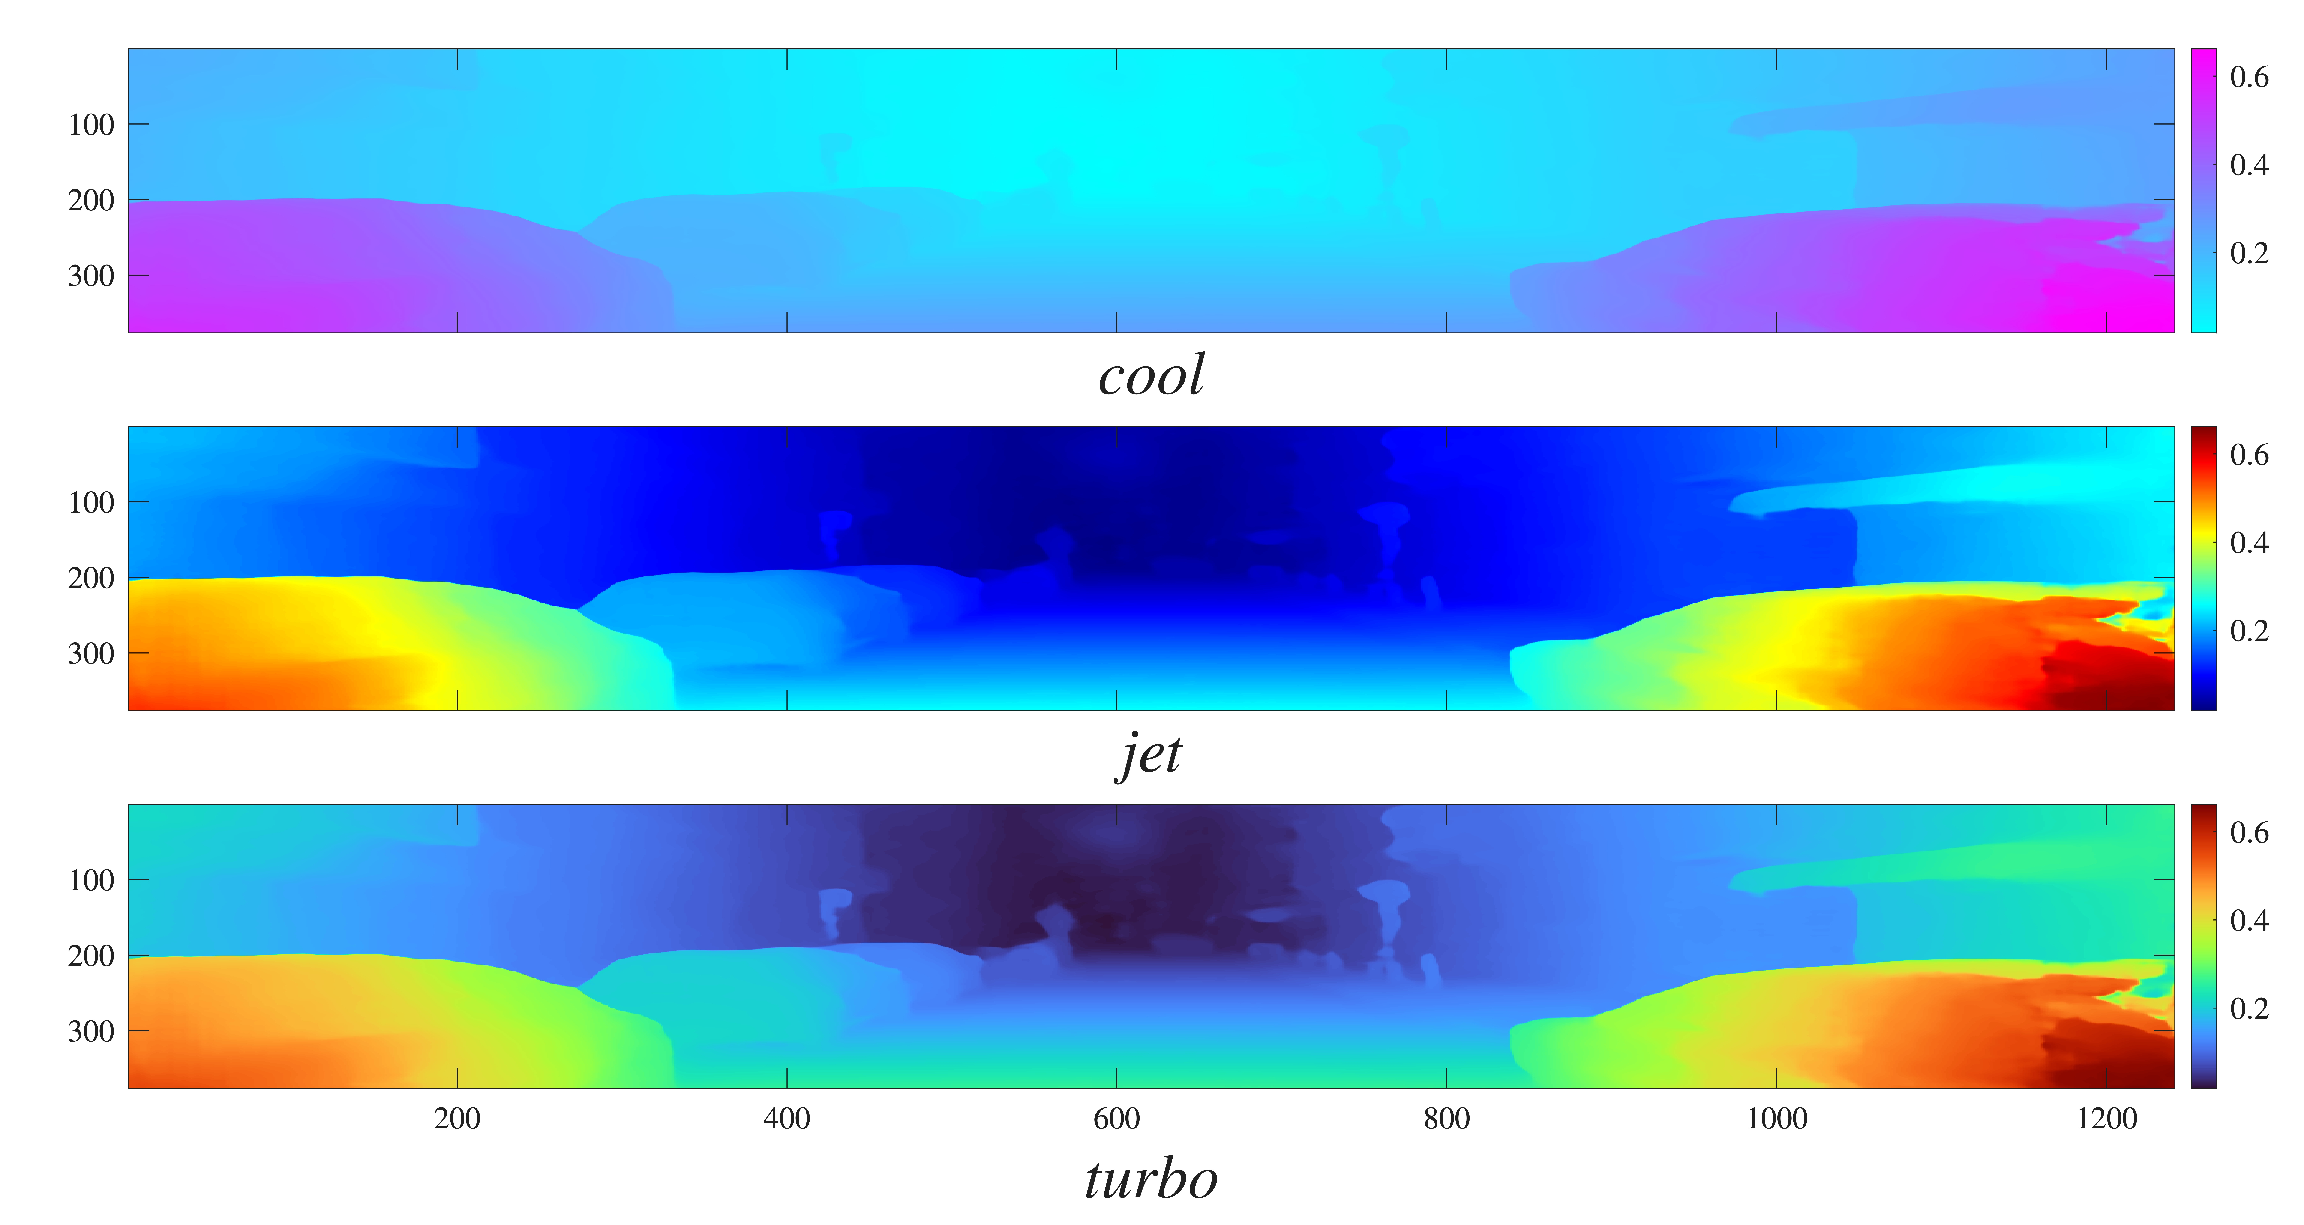
\includegraphics[width=0.80\linewidth]{Plots/images/dispRBG.pdf} \\
  % ---- Row 2 ----
  \rotatebox{90}{\makebox[6cm][c]{\emph{Row 2: colorblind}}}
  & 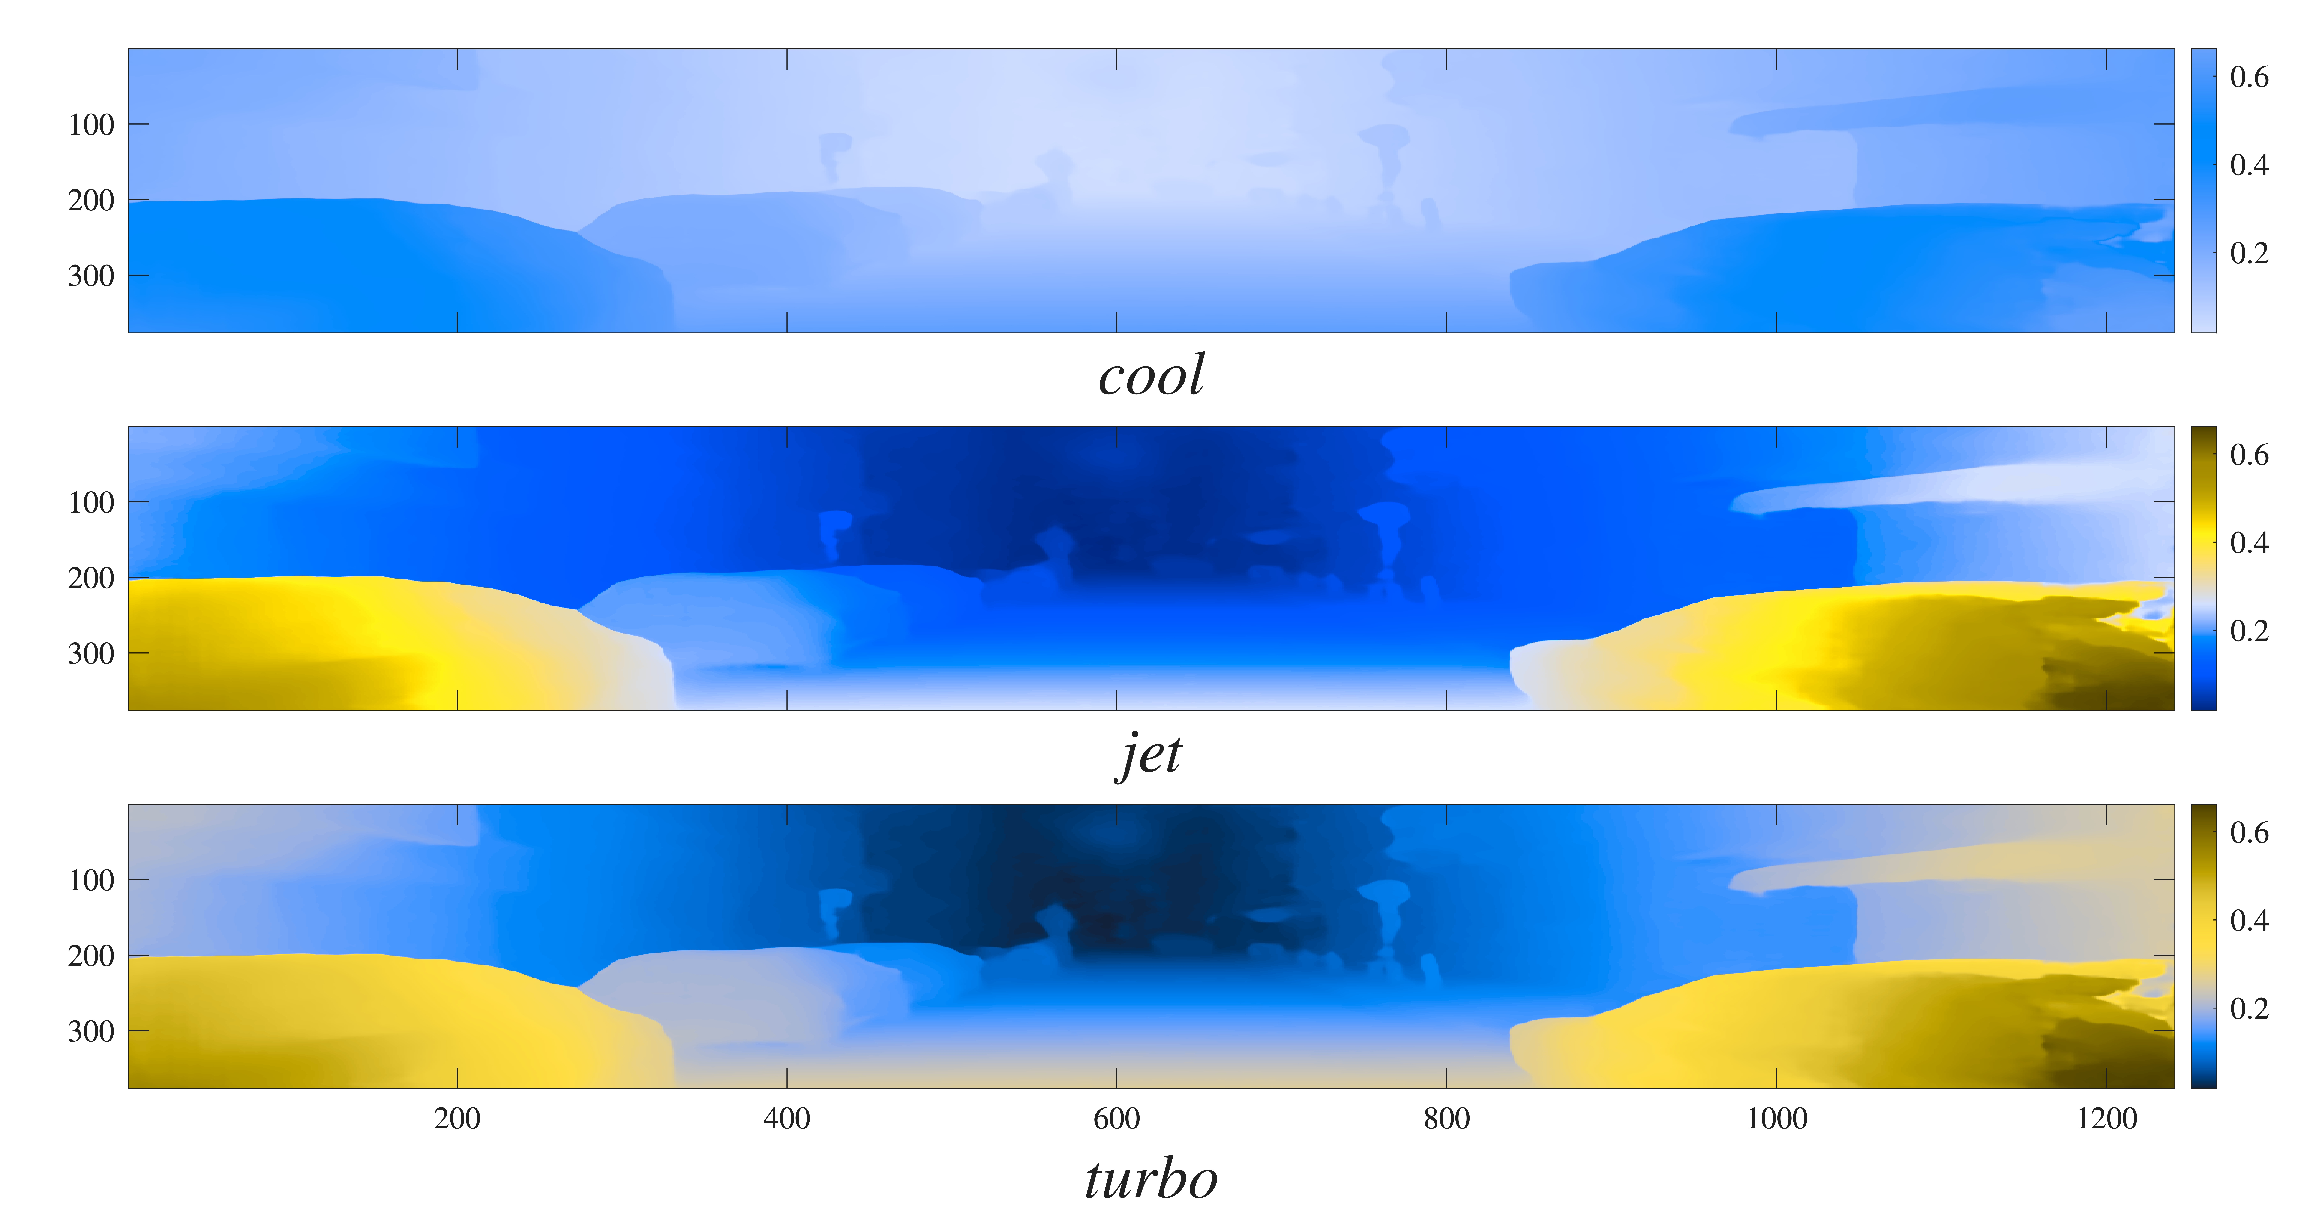
\includegraphics[width=0.80\linewidth]{Plots/images/dispProton.pdf} \\
  % ---- Row 3 ----
  \rotatebox{90}{\makebox[6cm][c]{\emph{Row 3: grayscale}}}
  & 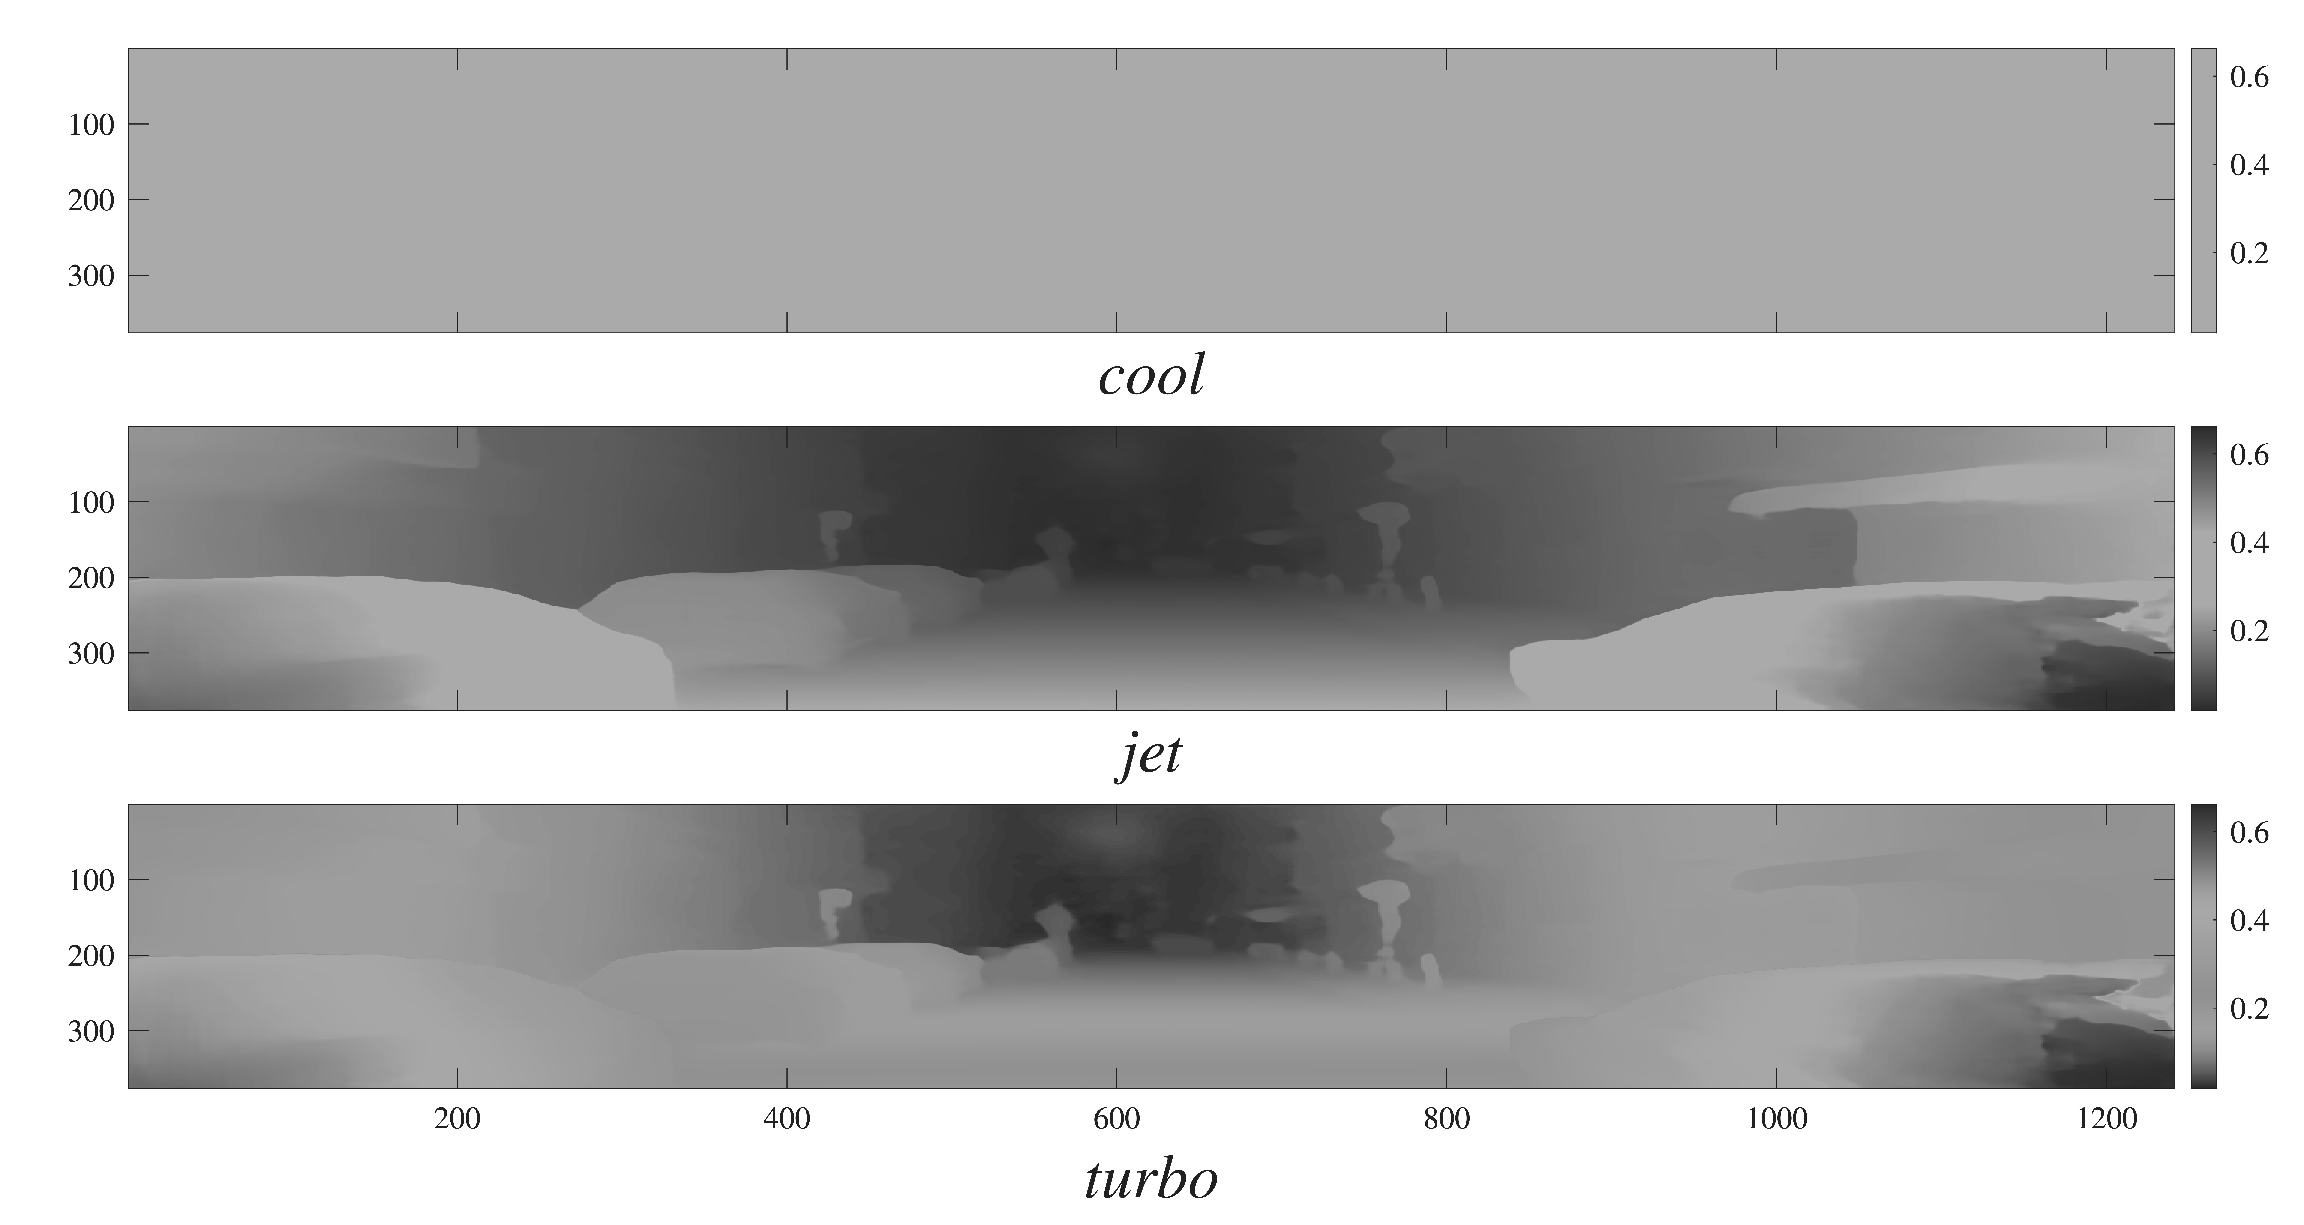
\includegraphics[width=0.80\linewidth]{Plots/images/dispMono.pdf} \\
\end{tabular}
\caption{wip}
\label{fig:fieldsPlots}
\end{framed}
\end{figure}

% { \Large \textcolor{magenta}{fix caption and once thats decided make as big as possible ALSO READ THRU CODE TO QC} }

\clearpage

% Now, let's consider . Each row of showcases the same data as that in  Figure~\ref{fig:exampField}, but with different colormaps. When choosing colormaps, it is important to consider both what is being presented and if the map is accessible. You may be drawn to the \textit{ice} colormap shown in row 1, as blue is a natural color choice for fluid or you enjoy it. However, \textit{ice} in grayscale washes out the gradient between the rings of "waves", making the field look more binary than connected. Row 2 shows \textit{jet}, once a quite popular colormap. You'll   

\section{Implementations}
\label{chpt:figCode}

{
\centering
\subsubsection{Lines in python}
\hrule{}
}

\begin{lstlisting}[language=python]
# plotting package import
import matplotlib.pyplot as plt
# numerics package import
import numpy as np

# LaTeX rendering in Latin Modern
plt.rcParams['text.usetex'] = True
plt.rcParams['text.latex.preamble'] = r'\usepackage{lmodern}'
plt.rcParams['font.family'] = 'serif'

# generate data
dxs = np.logspace(-4, 0, 40)  # grid spacings, 10^-4 to 10^0
y1 = 5.0*(dxs) + 8.0*(dxs**3)     # first order error curve
y2 = 2.0*(dxs**2) + 16.0*(dxs**4) # second order error curve

# reference lines (order one ref. is just dxs itself)
ref2 = dxs**2  # order two reference line

fs = 50  # set font size variable

# this is how you define non-standard colors! 
# all these values are the RBG #/255. this accepts both the 
# calculation (67/255) and the fraction (0.2627) for RBG triplets (see below)
badCols = np.array([
    [0.5, 0.000, 0.5],  # purple
    [0, 0, 0.9],        # blue
])


cols = np.array([
    [67/255, 179/255, 174/255],   # teal (marker edge/line 1)
    [136/255, 216/255, 192/255],  # light green (marker face 1)
    [198/255, 97/255, 166/255],   # light magenta (marker face 2)
    [202/255, 44/255, 146/255],   # magenta (marker edge/line 2)
])

# define figure, axes, and size
fig, ax = plt.subplots(figsize=(13, 9))

# bad color choice example (uses badCols)
# ax.plot(dxs, y1, '-', color=badCols[0, :])
# ax.plot(dxs, y2, '-', color=badCols[1, :])

# reference lines (excluded from legend)
ax.plot(dxs[:20], dxs[:20], '-.', color='black',
        linewidth=5, 
        label='_nolegend_') # this excludes this line from the legend
ax.plot(dxs[:20], 0.3*ref2[:20], '--', color='black',
        linewidth=5, label='_nolegend_')

# plots y1 vs dxs every third point as solid line with markers
ax.plot(dxs[::3], y1[::3], '-o',
        color=cols[0, :],            # set line color
        linewidth=2,                 # set line width
        markersize=24,               # set marker size
        markeredgewidth=3,           # set marker outline width
        markeredgecolor=cols[0, :],  # set marker outline color
        markerfacecolor=cols[1, :],  # set marker fill color
        label='first order')         # set legend entry

ax.plot(dxs[::3], y2[::3], '-*', color=cols[3, :], linewidth=2,
        markersize=40, markeredgewidth=3, markeredgecolor=cols[3, :],
        markerfacecolor=cols[2, :], label='second order')

# label reference slopes directly on the plot
ax.annotate(r'$\mathcal{O}(\Delta x)$',
            (1.3*dxs[5], 0.3*dxs[5]), fontsize=0.75*fs)
ax.annotate(r'$\mathcal{O}(\Delta x^2)$',
            (2.3*dxs[5], 0.4*(dxs[5]**2)), fontsize=0.75*fs)

# the multiplications you see above are simply translating the position to get 
# the labels off the line but close to it!

for spine in ax.spines.values():  # set axes line width
    spine.set_linewidth(3)
ax.tick_params(width=3, labelsize=fs)  # set tick width and font size
ax.tick_params(axis='x', pad=10)       # pad ticks away from axis (preventing overlap)

ax.set_xlabel(r'$\Delta x$  (mm)', fontsize=fs, labelpad=2)
ax.set_ylabel(r'Error', fontsize=fs)

ax.legend(fontsize=0.75*fs, loc='lower right')
ax.set_title('Convergence Plot', fontsize=fs)

# set the axis scale to log log
ax.set_xscale('log')
ax.set_yscale('log')
ax.grid() # sets major grid lines - can have settings here

# plt.show()  # uncomment to view interactively

## note: fig will not save if plt.show() is before plt.savefig(...)!!!!
# plt.savefig("linePlotExample.pdf", dpi=800)  # uncomment to export figure (dpi sets raster resolution)
\end{lstlisting}

{
\centering
\subsubsection{Fields in python}
\hrule
}

 \begin{lstlisting}[language=python]
# plotting package import
import matplotlib.pyplot as plt
# numerics package import
import numpy as np

# LaTeX rendering in Latin Modern
plt.rcParams['text.usetex'] = True
plt.rcParams['text.latex.preamble'] = r'\usepackage{lmodern}'
plt.rcParams['font.family'] = 'serif'

# generate data
dx = 0.01
x = np.arange(-np.pi, np.pi + dx, dx)  # + dx includes endpoint
y = x
X, Y = np.meshgrid(x, y) # creates mesh of x and y (2D fields)

# diverging colormap example (use cmap='PiYG' in pcolormesh)
###########################################################
R = np.sqrt(X**2 + Y**2)
f = Y * np.sin(2.0 * R**2)
###########################################################

# sequential colormap example (use cmap='Blues' in pcolormesh)
###########################################################
# f = R * 1.3**(1.01*(abs(abs(X)*abs(Y) - 2*np.pi)) + np.pi/2)
###########################################################

fs = 35  # set font size variable

fig, ax = plt.subplots(figsize=(12, 9))  # set figure size

ax.set_aspect('equal')  # force square aspect ratio

# pseudocolor plot of f across X and Y
# gouraud shading interpolates between cells (no mesh lines)
pc = ax.pcolormesh(X, Y, f, cmap='PiYG', shading='gouraud')

ax.set_xlabel('$x$', fontsize=fs)  # label x-axis in latex
ax.set_ylabel('$y$', fontsize=fs)  # label y-axis in latex

for spine in ax.spines.values():  # set axes line width
    spine.set_linewidth(3)
ax.tick_params(width=3, labelsize=fs)  # set tick width and font size

axesLims = [-np.pi, np.pi]  # define axes limits
ax.set_xlim(axesLims)       # set x axis limits
ax.set_ylim(axesLims)       # set y axis limits

cb = fig.colorbar(pc, ax=ax)                  # add colorbar
cb.ax.tick_params(labelsize=fs)               # set colorbar tick size
cb.set_label('Field Magnitude', fontsize=fs)  # label colorbar

# tick locations and latex labels
ticks = [-np.pi, -np.pi/2, 0, np.pi/2, np.pi]
tickLabel = ['$-\\pi$', '$-\\pi/2$', '$0$', '$\\pi/2$', '$\\pi$']

ax.set_xticks(ticks)           # set x tick locations
ax.set_yticks(ticks)           # set y tick locations
ax.set_xticklabels(tickLabel)  # set x tick labels to tex strings
ax.set_yticklabels(tickLabel)  # set y tick labels to tex strings

# plt.show()  # uncomment to view interactively

## note: fig will not save if plt.show() is before plt.savefig(...)!!!!
# plt.savefig("divergencePlotExample.pdf", dpi=800)  # uncomment to export figure 
# (dpi sets raster resolution)

#### 3D Plot

fig, ax = plt.subplots(subplot_kw={"projection": "3d"}, figsize=(12,9))

ax.plot_surface(X, Y, f, cmap=cm)

fs = 0.8*fs


ticks = [-np.pi, -np.pi/2, 0, np.pi/2, np.pi]  # defining location of ticks
tickLabel = ['$-\\pi$', '$-\\pi/2$', '$0$', '$\\pi/2$', '$\\pi$']  # defining labels for ticks

ax.set_xticks(ticks)            # set x ticks to ticks array
ax.set_yticks(ticks)            # set y ticks to ticks array
ax.set_xticklabels(tickLabel)   # set labels to tex strings in tickLabel
ax.set_yticklabels(tickLabel)   # set labels to tex strings in tickLabel


ax.set_xlabel('$x$', fontsize=fs, labelpad=20)  # label x-axis as x in latex
ax.set_ylabel('$y$', fontsize=fs, labelpad=20)
ax.set_ylabel('$f(x,y)$', fontsize=fs, labelpad=20)

for spine in ax.spines.values():   # set axes linewidth
    spine.set_linewidth(3)
ax.tick_params(width=3, labelsize=fs)  # set tick width and font size

axesLims = [-np.pi - 0.3, np.pi + 0.3]  # define axes limits
ax.set_xlim(axesLims)       # set x axis limits
ax.set_ylim(axesLims)       # set y axis limits

plt.show()

# plt.savefig("seq3D.pdf", dpi=800)
\end{lstlisting}


{
\centering
\subsubsection{Lines in MATLAB}
\hrule
}

 \begin{lstlisting}[language=matlab]

% generate data
dxs = logspace(-4, 0, 40);         % grid spacings, 10^-4 to 10^0

y1 = 5.0*dxs + 8.0*dxs.^3;         % first order error curve
y2 = 2.0*dxs.^2 + 16.0*dxs.^4;     % second order error curve

% reference lines (order one ref. is just dxs itself)
ref2 = dxs.^2;  % order two reference line

fs = 50;  % set font size variable

% rgb colors, defined 0-1
badCols = [0.5 0.0 0.5;    % purple
           0.0 0.0 0.9];   % blue

cols = [ 67 179 174;   % teal (marker edge/line 1)
        136 216 192;   % light green (marker face 1)
        198  97 166;   % light magenta (marker face 2)
        202  44 146] / 255;  % magenta (marker edge/line 2)

% define figure, axes, and size
fig = figure( ...
    "Theme", "light", ...               % plot light even in dark mode
    'Position', [100, 100, 1300, 900]); % match figsize(13,9)

hold on  % ensures all following plot commands go onto fig

% bad color choice example (uses badCols)
% plot(dxs, y1, '-', 'Color', badCols(1,:))
% plot(dxs, y2, '-', 'Color', badCols(2,:))

% reference lines (excluded from legend, truncated to lower half)
plot(dxs(1:20), dxs(1:20), '-.', 'Color', 'black', ...
    'LineWidth', 5, 'HandleVisibility', 'off')
plot(dxs(1:20), 0.3*ref2(1:20), '--', 'Color', 'black', ...
    'LineWidth', 5, 'HandleVisibility', 'off')

% plots y1 vs dxs every third point as solid line with markers
plot(dxs(1:3:end), y1(1:3:end), '-o', ...
    'Color', cols(1,:), ...            % set line color
    'LineWidth', 2, ...                % set line width
    'MarkerSize', 24, ...              % set marker size
    'MarkerEdgeColor', cols(1,:), ...  % set marker outline color
    'MarkerFaceColor', cols(2,:), ...  % set marker fill color
    'DisplayName', 'first order')      % set legend entry

plot(dxs(1:3:end), y2(1:3:end), '-p', 'Color', cols(4,:), ...
    'LineWidth', 2, 'MarkerSize', 40, ...
    'MarkerEdgeColor', cols(4,:), 'MarkerFaceColor', cols(3,:), ...
    'DisplayName', 'second order')

% label reference slopes directly on the plot
text(1.3*dxs(6), 0.3*dxs(6), '$$\mathcal{O}(\Delta x)$$', ...
    'Interpreter', 'latex', 'FontSize', 0.75*fs)
text(2.3*dxs(6), 0.4*dxs(6)^2, '$$\mathcal{O}(\Delta x^2)$$', ...
    'Interpreter', 'latex', 'FontSize', 0.75*fs)

ax = gca;  % pull the current axes
set(ax, ...
    'XScale', 'log', ...              % set x-scale to log
    'YScale', 'log', ...              % set y-scale to log
    'LineWidth', 3, ...               % set axes line width
    'FontSize', fs, ...               % set tick font size
    'TickLabelInterpreter', 'latex'); % set tick interpreter to latex

grid on  % turn on major grid

xlabel('$$\Delta x$$  (mm)', ...  % label x-axis in latex
    'Interpreter', 'latex', ...   % interpret label with latex
    'FontSize', fs);              % set font size of label

ylabel('Error', 'Interpreter', 'latex', 'FontSize', fs);

legend('FontSize', 0.75*fs, ...   % set legend font size
    'Location', 'southeast', ...  % legend bottom right
    'Interpreter', 'latex');      % interpret with latex

title('Convergence Plot', ...    % set plot title
    'Interpreter', 'latex', ...  % interpret title in latex
    'FontSize', fs);             % set font size of title

hold off

saveas(fig, 'convergencePlot.pdf')  % export figure as a pdf




\end{lstlisting}

{
\centering
\subsubsection{Fields in MATLAB}
\hrule
}
 \begin{lstlisting}[language=matlab]

% point matlab to any cmap directories you download
% needed for curl and blues
addpath('<path to directory>/cmap/')

cm = curl(256);

% generate data
dx = 0.01;
x = -pi:dx:pi;
y = x;
[X, Y] = meshgrid(x, y);  % creates mesh of x and y (2D fields)

% diverging colormap example (use colormap('curl'))
%%%%%%%%%%%%%%%%%%%%%%%%%%%%%
R = sqrt(X.^2 + Y.^2);
f = Y.*sin(2.0*R.^2);
%%%%%%%%%%%%%%%%%%%%%%%%%%%%%

% sequential colormap example (use colormap('Blues'))
%%%%%%%%%%%%%%%%%%%%%%%%%%%%%
% f = R .* 1.3.^(1.01*(abs(abs(X).*abs(Y) - 2*pi)) + pi/2);
%%%%%%%%%%%%%%%%%%%%%%%%%%%%%

 % set colormap to match the example above

fs = 35;  % set font size variable

fig = figure( ...
    "Theme", "light", ...               % plot light even in dark mode
    'Position', [100, 100, 1200, 900]); % match figsize(12,9)

hold on  % ensures all following plot commands go onto fig

daspect([1 1 1])  % force square aspect ratio

% pseudocolor plot of f across X and Y
pc = pcolor(X, Y, f);
colormap(cm);
shading interp     % interpolate between cells (matches gouraud)


xlabel('$$x$$', ...              % label x-axis in latex
    'Interpreter', 'latex', ...  % interpret label with latex
    'FontSize', fs);             % set font size of label

ylabel('$$y$$', 'Interpreter', 'latex', 'FontSize', fs);

ax = gca;  % pull the current axes
set(ax, 'LineWidth', 3, 'FontSize', fs)  % set axes width, font size

axesLims = [-pi, pi];  % define axes limits
xlim(axesLims)         % set x axis limits
ylim(axesLims)         % set y axis limits

cb = colorbar('TickLabelInterpreter', 'latex', ...  % add colorbar
    'FontSize', fs);                                % set tick size
ylabel(cb, 'Field Magnitude', ...  % label colorbar
    'FontSize', fs, ...            % set font size
    'Interpreter', 'latex');       % set label interpreter

% tick locations and latex labels
ticks = [-pi, -pi/2, 0, pi/2, pi];
tickLabel = {'$$-\pi$$', '$$-\pi/2$$', '$$0$$', ...
             '$$\pi/2$$', '$$\pi$$'};

ax.TickLabelInterpreter = 'latex';  % set tick interpreter to latex
ax.XTick = ticks;                   % set x tick locations
ax.YTick = ticks;                   % set y tick locations
ax.XTickLabel = tickLabel;          % set x tick labels to tex strings
ax.YTickLabel = tickLabel;          % set y tick labels to tex strings

hold off

%% note: exports whatever figure is current!
% exportgraphics(fig, 'div.pdf', 'Resolution', 800)

%%---------------------------
%% 3D PLOT
%%---------------------------

fig = figure( ...
    "Theme", "light", ...               % plot light even in dark mode
    'Position', [100, 100, 1200, 900]); % match figsize(12,9)

% surface plot of f across X and Y
s = surf(X, Y, f, 'EdgeColor', 'none'); % EdgeColor none removes mesh lines
colormap(cm);  % set colormap (cm defined above)

fs = 0.8*fs;  % shrink fonts for the 3d view

% tick locations and latex labels
ticks = [-pi, -pi/2, 0, pi/2, pi];
tickLabel = {'$$-\pi$$', '$$-\pi/2$$', '$$0$$', ...
             '$$\pi/2$$', '$$\pi$$'};

ax = gca;  % pull the current axes
ax.TickLabelInterpreter = 'latex';  % set tick interpreter to latex
ax.XTick = ticks;                   % set x tick locations
ax.YTick = ticks;                   % set y tick locations
ax.XTickLabel = tickLabel;          % set x tick labels to tex strings
ax.YTickLabel = tickLabel;          % set y tick labels to tex strings

xlabel('$$x$$', ...              % label x-axis in latex
    'Interpreter', 'latex', ...  % interpret label with latex
    'FontSize', fs);             % set font size of label

ylabel('$$y$$', 'Interpreter', 'latex', 'FontSize', fs);
zlabel('$$f(x,y)$$', 'Interpreter', 'latex', 'FontSize', fs);

set(ax, 'LineWidth', 3, 'FontSize', fs)  % set axes width, font size

axesLims = [-pi - 0.3, pi + 0.3];  % define axes limits (small margin)
xlim(axesLims)                     % set x axis limits
ylim(axesLims)                     % set y axis limits

%% note: exports whatever figure is current!
% exportgraphics(fig, 'seq3D.pdf', 'Resolution', 800)

\end{lstlisting}





% \begin{wrapfigure}{r}{6.2cm}
%   \vspace*{-0.7cm}
% \begin{framed}

%   % (\emph{a})
%   % \hspace*{3cm}
%   % (\emph{b})\\[1mm]
%   % \hspace*{-4mm}
%   \includegraphics[trim = 0mm 0mm 0mm 0mm,clip,width=5.5cm, page=2]{Plots/images/compCMAP.pdf}
%     \includegraphics[trim = 0mm 0mm 0mm 0mm,clip,width=5.5cm, page=1]{Plots/images/compCMAP.pdf}
%   \\ [-8mm]
%   \caption{\textcolor{magenta}{fix}}
%   \vspace*{-2mm}
%   \label{fig:exampField}
% \end{framed}
% \end{wrapfigure} 
\chapter{Finite Difference Methods}
\label{chpt:FDM}

Finite difference methods (FDM) are collocation methods based on Taylor
series approximation and are used to approximate derivatives and derivative operators. They are an old and simple numerical method which became popular after the development as computers due to the sheer amount of arithmetic for application. In this chapter, we will define numerical schemes to approximate first and second derivatives. These schemes can then be extended to help solve PDEs by approximating derivatives and derivative operators ($\nabla, \nabla^2$).
\index{finite difference methods}
\section{The Basics}

\begin{wrapfigure}{r}{0.4\textwidth}
\centering
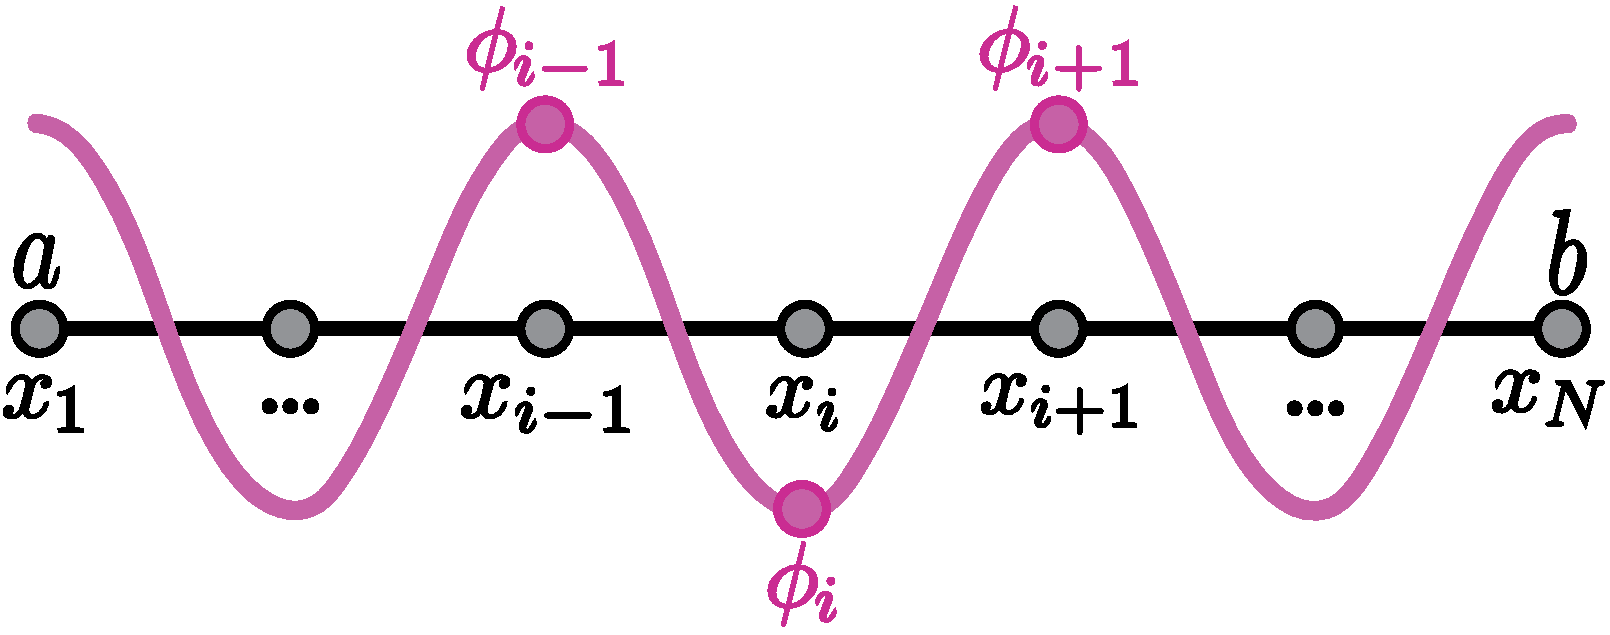
\includegraphics[width=0.38\textwidth, page=1]{FDM/images/1DFDMv6.pdf}
\caption{A smooth function $\phi$ sampled on the equally spaced grid
$\{x_i\}$ partitioning $[a,b]$. $\phi$ is discretely sampled on the grid, where
$\phi_i \equiv \phi(x_i)$ .}
\label{fig:grid}
\end{wrapfigure}


Consider a domain $[a,b]\subset\mathbb{R}$ and a grid of
equally spaced points $\{x_i\}_{i=0}^{N}\subset[a,b]$ such that $x_0=a$ and
$x_N=b$. The spacing between neighboring points can be computed as
$
\Delta x = \frac{b-a}{N}
$
so that $x_i = a + i\,\Delta x$. Given some function $\phi: [a,b] \to\mathbb{R}$, we denote
$\phi_i \equiv \phi(x_i)$. 
 

 
Recall that a sufficiently smooth function can be written as a Taylor series about a single point. Assuming $\phi$ is smooth, its Taylor series about some point $x_i$ is
\begin{equation}
\phi(x) = \phi_i + \phi'_i\,\Delta x
+ \frac{\phi''_i}{2}\,\Delta x^2 + \cdots
\label{eq:taylorForward}
\end{equation}
\index{Taylor series}
for $x \in [a,b]$. The finite difference approach evaluates $\phi$ at respective $x \in \{x_i\}_{i =0}^{N}$ in terms of a Taylor series about one of its neighbors (i.e., $\phi_{i}$), where the series can be truncated for sufficiently small $\Delta x$. The remaining series terms are rearranged to produce approximations for various derivatives with well-defined error from the truncated terms. 

\section{First Derivative Approximations}
\index{finite difference methods!first derivatives}
\label{sec:firstderiv}
We will discuss the forward,
backward, and central difference scheme for approximating $\phi'_i$. The former two are first-order schemes and the latter is second-order.
\index{finite difference methods!first derivatives!forward difference}

To discuss finite difference schemes, we will adopt the compass notation. For a grid point of interest $P$,
its neighbor to the west (decreasing $x$) is $W$ and its neighbor to the
east (increasing $x$) is $E$. 

\subsection{Forward difference}
Following from \eqref{eq:taylorForward}, $\phi_{i + 1}$ can be approximated as 
$$
\phi_{i + 1} = \phi_i + \phi'_i \Delta x + \frac{\phi''_i}{2} (\Delta x^2) + \hdots 
$$
Solving this approximation for $\phi'_i$ yields
\[
\phi'_i = \frac{\phi_{i+1}-\phi_i}{\Delta x} - R,
\qquad
R = \frac{\phi''_i}{2}\,\Delta x + \hdots,
\]
where $R$ is the local truncation error. The magnitude of error $R$ is controlled by the leading
retained term $\tfrac{1}{2}\phi''_i\,\Delta x$, which is proportional to
$\Delta x$. This error is generally recorded using Big~$\mathcal{O}$ notation,
\begin{equation}
\phi'_i = \frac{\phi_{i+1}-\phi_i}{\Delta x} + \mathcal{O}(\Delta x), \quad \phi'_P = \frac{\phi_{E}-\phi_P}{\Delta x} + \mathcal{O}(\Delta x),
\label{eq:fdFO1}
\end{equation}
Equation~\eqref{eq:fdFO1} is the \emph{first-order forward
difference} approximation of $\phi'_i$ and the points of interest are highlighted in Figure~\ref{fig:forwardDiff}. The word forward refers to the fact that
the Taylor series around $x_i$ estimates $\phi$ at the next or forward point $x_{i+1}$. Note how derivative approximation resembles the limit
definition of the derivative!

\begin{figure}[htbp]
    \centering
    \includegraphics[width=0.33\textwidth, page=7]{FDM/images/1DFDMv6.pdf}
    \caption{The forward difference stencil, highlighting the used points $P, E$ in cyan. }
    \label{fig:forwardDiff}
\end{figure}

\index{finite difference methods!first derivatives!backward difference}

\subsection{Backward difference}
Estimating the previous point $\phi_{i - 1}$ in terms of \eqref{eq:taylorForward} yields
\begin{equation}
\phi_{i - 1} = \phi_i - \phi'_i\,\Delta x
+ \frac{\phi''_i}{2}\,\Delta x^2
- \frac{\phi'''_i}{6}\,\Delta x^3 + \cdots,
\label{eq:taylorBackward}
\end{equation}
The odd terms of the series are now negative, as $(x_i - \Delta x) - x_i = -\Delta x$. Solving \ref{eq:taylorBackward} for $\phi'(x_i)$ gives the \emph{first-order backward difference},
\begin{equation}
\phi'(x_i) = \frac{\phi_i-\phi_{i-1}}{\Delta x} + \mathcal{O}(\Delta x), \quad \phi'(x_P) = \frac{\phi_P-\phi_{W}}{\Delta x} + \mathcal{O}(\Delta x).
\label{eq:fdBO1}
\end{equation}

\begin{figure}[htbp]
    \centering
    \includegraphics[width=0.33\textwidth, page=4]{FDM/images/1DFDMv6.pdf}
    \caption{The backward difference stencil, highlighting the used points $P, W$ in cyan. }
    \label{fig:backwardDiff}
\end{figure}

The stencil for this scheme is showcased in Figure~\ref{fig:backwardDiff}. The word backwards refers to the fact that
the Taylor series around $x_i$ estimates $\phi$ at the last or backward point $x_{i-1}$.

\index{finite difference methods!first derivatives!central difference}
\subsection{Central difference}
\label{sec:central}
Reorganizing the forward and backwards Taylor series approximations yields
\begin{align}
\phi'_i &=  \frac{\phi_{i+1}-\phi_i}{\Delta x} - \frac{\phi''_i}{2}\,\Delta x - \frac{\phi'''_i}{3}\,\Delta x^2 + \cdots \label{eq:add1}
\\
 \phi'_i &= \frac{\phi_i-\phi_{i-1}}{\Delta x}  + \frac{\phi''_i}{2}\,\Delta x - \frac{\phi'''_i}{3}\,\Delta x^2 + \cdots \label{eq:add2}
\end{align}
Adding  \eqref{eq:add1} and \eqref{eq:add2} and dividing by a factor of two obtains a second-order accurate scheme:
\begin{equation}
\phi'(x_i) = \frac{\phi_{i+1}-\phi_{i-1}}{2\,\Delta x} - \frac{\phi'''(x_i)}{6}\,\Delta x^2 + \cdots = \frac{\phi_{i+1}-\phi_{i-1}}{2\,\Delta x} + \mathcal{O}(\Delta x^2).
\label{eq:fdCentral}
\end{equation}

Using our compass notation, the central difference scheme is written as 
$$
\phi'(x_P) = \frac{\phi_{E}-\phi_{W}}{2\,\Delta x} + \mathcal{O}(\Delta x^2).
$$
This stencil is highlighted in Figure~\ref{fig:centralDiff}.

\begin{figure}[htbp]
    \centering
    \includegraphics[width=0.33\textwidth, page=8]{FDM/images/1DFDMv6.pdf}
    \caption{The central difference stencil, highlighting the used points $E, W$ in cyan. }
    \label{fig:centralDiff}
\end{figure}


\section{Second Derivative Approximations}
\label{sec:secondderiv}
\index{finite difference methods!second derivatives!central difference}
To approximate $\phi''_i$ we estimate in the forward and backward directions:
\begin{align}
\phi_{i+1} &= \phi_i + \phi'_i\,\Delta x
+ \frac{\phi''_i}{2}\,\Delta x^2
+ \frac{\phi'''_i}{6}\,\Delta x^3
+ \frac{\phi''''_i}{24}\,\Delta x^4 + \cdots, \label{eq:add11}\\
\phi_{i-1} &= \phi_i - \phi'_i\,\Delta x
+ \frac{\phi''_i}{2}\,\Delta x^2
- \frac{\phi'''_i}{6}\,\Delta x^3
+ \frac{\phi''''_i}{24}\,\Delta x^4 - \cdots. \label{eq:add22}
\end{align}
Adding \eqref{eq:add11} and \eqref{eq:add22}, the odd-order terms cancel and
\[
\phi_{i+1}+\phi_{i-1} = 2\,\phi_i + \phi''_i\,\Delta x^2
+ \frac{\phi'''_i}{12}\,\Delta x^4 + \cdots.
\]
\vspace*{-2mm}
Solving for $\phi''_i$ gives the second-order central
difference scheme for the second derivative:
\begin{equation}
\phi''_i = \frac{\phi_{i+1} - 2\phi_i + \phi_{i-1}}{\Delta x^2}
+ \mathcal{O}(\Delta x^2).
\label{eq:fdSecond}
\end{equation}


On their own, these approximations only tell us how
$\phi$ changes locally; to actually solve a differential equation
we must define how $\phi$ behaves at the edges of the domain through \emph{boundary conditions} which rely on \emph{ghost points}. We will use an example problem in the next section to define two styles of spatial discretization and how to use ghost points to define boundary conditions.

\chapter{One-Dimensional FDMs in Practice}
\label{sec:bvp-example}

Consider the second-derivative operator $D_{xx} \equiv \frac{d^2}{dx^2}$
acting on a smooth function $\phi : [a,b] \to \mathbb{R}$. We want to use finite difference methods to solve the following for $\phi$:
\begin{equation}
    D_{xx}\phi = -\sin(x), \qquad x \in [a,b]
    \label{eq:bvp-model}
\end{equation}
Equation~\eqref{eq:bvp-model} tells us that the second
derivative of $\phi$ equals $f(x) = -\sin(x)$. Integrating $f$ twice reveals that
\begin{align}
    \phi'(x) &= \cos(x) + c_1, \\
    \phi(x)  &= \sin(x) + c_1\,x + c_2,
    \label{eq:bvp-general}
\end{align}
where $c_1, c_2 \in \mathbb{R}$ are constants of integration. Notice that
\eqref{eq:bvp-general} is not a single solution but an entire
two-parameter family: any choice of $c_1$ and $c_2$ satisfies
\eqref{eq:bvp-model}. 


\begin{remark}
To single out a solution we must supply extra pieces of
information through boundary conditions.
\index{boundary conditions}
\end{remark}

Boundary conditions are almost always imposed at the ends of the domain, which are $x=a$ and $x=b$ for this problem. For example, on $[a,b] = [0, 2\pi]$ with the conditions $\phi(0)=0$ and
$\phi(2\pi)=0$, the two constants in \eqref{eq:bvp-general} are forced to
$c_1 = c_2 = 0$, leaving the unique exact solution $\phi(x) = \sin(x)$.
We will return to this case as a convenient way to check our numerical
schemes.

We can think about this need for boundary conditions in terms of our discrete grid as well. Suppose we sample $\phi$ on the equally spaced grid seen in Figure~\ref{fig:standardgrid} and approximate
$D_{xx}\phi$ at each grid point $P$ using the second-order central difference
\begin{equation}
    D_{xx}\phi\big|_{P}
    \;\approx\;
    \frac{\phi_{E} - 2\phi_P + \phi_{W}}{\Delta x^2},
    \label{eq:bvp-central}
\end{equation}

we would end up with this linear system:
\begin{equation}
    \frac{1}{\Delta x^2}
    \begin{bmatrix}
        ? & ? & ?& ?& \cdots & ?\\
        1 & -2 & 1 &0 &\cdots & 0 \\
         \vdots & \ddots & \ddots & \ddots & \ddots & \vdots\\
          \vdots & \ddots & \ddots & \ddots & \ddots & \vdots\\
          0&\cdots & 0 & 1 & -2 & 1 \\
          ?&\cdots & ? & ?& ? & -?
    \end{bmatrix}
    \begin{bmatrix}
        \phi_0 \\ \phi_1 \\ \vdots \\ \vdots \\ \phi_{N-1} \\ \phi_N
    \end{bmatrix}
    =
    \begin{bmatrix}
        -\sin(x_0)  \\
        -\sin(x_2) \\
        \vdots \\
                \vdots \\
        -\sin(x_{N-1}) \\
        -\sin(x_N) 
    \end{bmatrix}.
    \label{baseFDM}
\end{equation}


\begin{figure}[htbp]
    \centering
    \includegraphics[width=0.9\textwidth, page=9]{FDM/images/1DFDMv6.pdf}
    \caption{A standard grid discretization of some real-valued domain $[a,b]$. The domain is discretized by $N +1$ equally-spaced points a distance $\Delta x$ apart. Exterior points (orange) at domain boundaries $x=a,b$ highlighted, as well as ghost points $x_{-1}$ and $x_{N + 1}$.}
    \label{fig:standardgrid}
\end{figure}

At any \emph{interior} (cyan) point the three values $W, P, E$
are all available and \eqref{eq:bvp-central} is well defined. But at the
\emph{exterior} (orange) grid points $x_0$ and $x_N$, the stencil calls for $\phi_{-1}$ and $\phi_{N+1}$... these values lie outside the grid! The linear system is then left with more unknowns than equations, so our linear system is under-determined\footnote{Note that if we were to not notice this, and set $D_{xx}(0,0) = 2, D_{xx}(0, 1) = -1,$ etc., the system would solve and give a real solution. Consider why this is, and determine what it implies about the boundaries!}. To create a well-determined system and force a unique solution, we must define these values that lie outside the grid, which we call \emph{ghost points}. Note that one could instead use first-order one-sided differences at the boundaries, but this lowers the order of the boundary approximation and can degrade the accuracy of the whole scheme, so it is generally avoided in favor of the ghost-point construction.

Where these ghost point actually sits depends on how we lay the grid down
relative to the boundary. The next two sections describe the two standard
choices for grids.

\index{ghost points}


\section{Type I Grids}
\label{sec:typeI}

A \textbf{Type I} (or \emph{nodal}, \emph{vertex-centered}) grid places
discrete points \emph{on} the boundaries $a,b$. We have been already thinking about discretization on a Type I grid, which defines discrete points $x_i \in [a,b]$ as
\begin{equation}
    x_i = a + i\,\Delta x, \quad i = 0,1,\dots,N,
    \qquad \Delta x = \frac{b-a}{N},
\end{equation}
so that $x_0 = a$ and $x_N = b$ are themselves grid points. The ghost
points are the two nodes obtained by stepping one $\Delta x$ past each end,
\begin{equation}
    x_{-1} = a - \Delta x, \qquad x_{N+1} = b + \Delta x,
\end{equation}
shown as the grey or first/last points in Figure~\ref{fig:typeI}. At the left boundary $x = a$ we can lay our finite difference stencil, seen as the shaded region, where
$P = x_0$, $W = x_{-1}$, and $E = x_1$. The same idea can be applied to the right boundary $x = b$, where $P = x_N$, $E = x_{N+1}$, and $W = x_{N-1}$.
\index{nodal grid}\index{grid!Type I}

\begin{figure}[htbp]
    \centering
    \includegraphics[width=0.9\textwidth, page=3]{FDM/images/1DFDMv6.pdf}
    \caption{A Type~I (nodal) grid on $[a,b]$. Interior points $x_1, \hdots, x_{N - 1}$ seen in lighter cyan and exterior points $x_0, x_N$ seen as darker orange. Ghost nodes are first and last points defined in gray and black. Finite different stencil for $P = x_0$ highlight as grey stroke, with contributors $P, E,$ and $W$ labelled.}
    \label{fig:typeI}
\end{figure}

A defining feature of a Type~I grid is that implementing boundary conditions is direct, since
the boundary value is a nodal value.

\section{Type II Grids}
\label{sec:typeII}

A \textbf{Type II} (or \emph{cell-centered}) grid instead partitions
$[a,b]$ into $N$ \textbf{cells} of width $\Delta x = \tfrac{b-a}{N}$ and
places the discrete points of $x$ at the cell \emph{centers}. This results in one less discrete point when compared to Type I grids. The cell
\emph{faces} fall on the boundaries, so no discrete point $x$ lies on the domain
edge. The cell centers are
\begin{equation}
    x_{i + 1/2} = a + \left(i + \tfrac{1}{2}\right)\Delta x,
    \quad i = 0,1,\dots,N - 1
\end{equation}
and the faces still sit at $x_{i} = a + i\,\Delta x$. This cell idea is depicted for the discrete point $x_i$ in Figure~\ref{fig:typeII}. The two boundaries still sit at $x_0$ and $x_N$, but the nearest grid point is half a spacing away. The ghost points lie half a spacing outside each end of the domain,
as seen by the gray and black crosses in Figure~\ref{fig:typeII}. At the left boundary, we can lay our finite difference stencil, seen as the gray shaded region, where $P = x_{1/2}$, $W = x_{-1/2}$, and $E = x_{3/2}$, and the boundary itself is the west face of $x_{1/2}$ and east face of $x_{-1/2}$.
\index{cell-centered grid}\index{grid!Type II}

\begin{figure}[htbp]
    \centering
    \includegraphics[width=0.9\textwidth, page=10]{FDM/images/1DFDMv6.pdf}
    \caption{A Type~II (cell-centered) grid on $[a,b]$ shown as stars. Interior points $x_{3/2}, \hdots, x_{N - 3/2}$ seen in lighter cyan and exterior points $x_{1/2}, x_{N-1/2}$ seen as darker orange. Ghost nodes are first and last points defined in gray and black. Finite different stencil for $P = x_{1/2}$ highlight as grey stroke, with contributors $P, E,$ and $W$ labelled. The cell definition is labelled for $x_{i + 1/2}$, with the diameter $\Delta x$ and region referred to as the cell face labelled.}
    \label{fig:typeII}
\end{figure}

A defining feature for Type~II grids is that the domain boundaries sit
\emph{exactly halfway} between the ghost points and the corresponding interior point. A difference across $W$ and $P$ is therefore naturally centered
on the boundary. We will discuss later that layout makes first-order methods
second-order accurate at the cell faces without any extra work.

\section{Boundary Conditions}
\label{sec:bcs}

We will now define the three boundary conditions used in this text and, for
each, give the ghost value it implies on both grid types. Throughout we
write the prescribed left-boundary value as $\alpha \in \mathbb{R}$ and the right-boundary
value as $\beta  \in \mathbb{R}$, and derive the left boundary in detail. The right
boundary follows by symmetry and is left as an exercise.

\subsection{Periodic Boundaries}
\label{sec:bc-periodic}

A \textbf{periodic} boundary condition treats the domain as a loop: the solution $\phi$
and its derivatives at $x=a$ match those at $x=b$. This is implemented by setting ghost points as the opposite end of the domain.
\index{periodic boundary condition}\\

\paragraph{Type~I.} Because the nodes $x_0=a$ and $x_N=b$ represent the same
physical location, we carry the $N$ distinct unknowns
$\phi_0,\dots,\phi_{N-1}$ and remove $\phi_N \equiv \phi_0$ from our system as a known value. Stepping
west past the first node wraps around to the last interior node, so the
ghost is
\begin{equation}
    \phi_W = \phi_{-1} \equiv \phi_{N-1}.
\end{equation}
For the first row of the system~\ref{baseFDM}, this would look like 
\begin{equation}
    \frac{1}{\Delta x^2}
    \begin{bmatrix}
        -2 & 1 & 0& 0& \cdots & 0 & 1\\
    \end{bmatrix}
    \begin{bmatrix}
        \phi_0 & \phi_1 &  \phi_2 & \phi_3 &  \cdots & \phi_{N-1}
    \end{bmatrix}^T
    =
    \begin{bmatrix}
        -\sin(x_1)
    \end{bmatrix}. \label{periodQueen}
\end{equation}


\paragraph{Type~II.} The cells wrap directly: the left ghost cell is a copy of
the last interior cell and the right ghost cell is a copy of the first,
\begin{equation}
    \phi_W = \phi_{-1/2} \equiv \phi_{N-1/2}
\end{equation}
This would be imposed just the same as \eqref{periodQueen}.
\subsection{Dirichlet}
\label{sec:bc-dirichlet}


A \textbf{Dirichlet} boundary condition prescribes a \emph{value} $\alpha$ of $\phi$ at
the boundary, such that $\phi(a) = \alpha$. Consider how this might be described in two different ways within our linear system for the Type I grid, and why there is only one method for a Type II grid.
\index{Dirichlet boundary condition} \\

\paragraph{Type~I.} The boundary value lives at the node $P = x_0$, so it is
imposed directly,
\begin{equation}
    \phi_P = \alpha .
\end{equation}
One method for implementing this condition is by writing the first row of the system~\eqref{baseFDM} as 

\begin{equation}
    \frac{1}{\Delta x^2}
    \begin{bmatrix}
        1& 0 & \cdots & 0\\
    \end{bmatrix}
    \begin{bmatrix}
        \phi_0 & \phi_1 &  \cdots  & \phi_N
    \end{bmatrix}^T
    =
    \begin{bmatrix}
        \alpha
    \end{bmatrix}. \label{basicDir}
\end{equation}

\noindent Alternatively, we can treat $\phi_0 = \alpha$ and $\phi_N = \beta$ as known and
remove them from the unknowns, leaving a linear system for $\phi_1,\dots,\phi_{N-1}$ and removing the first and last rows of the system~\eqref{baseFDM}. Moving the
known value across the linear system, the (now first) row for $\phi_1$ becomes
\begin{equation}
    \frac{1}{\Delta x^2}
    \begin{bmatrix}
        -2& 1 & 0 & \cdots & 0\\
    \end{bmatrix}
    \begin{bmatrix}
        \phi_1 & \phi_2 & \phi_3 &  \cdots  & \phi_{N-1}
    \end{bmatrix}^T
    =
    \begin{bmatrix}
        -\sin(x_1) - \frac{\alpha}{\Delta x^2}
    \end{bmatrix}. \label{rhsDirTop}
\end{equation}
Both methods are equivalent.

\paragraph{Type~II.} 
On a Type~II grid there is no discrete point at the boundary, so we can only implement the condition on the right-hand side of our linear system. We approximate the boundary as the midpoint between $x_{-1/2}$ and $x_{1/2}$:
$$
\alpha = \frac{\phi_{-1/2} + \phi_{1/2}}{2} \implies \phi_{-1/2} = 2\alpha - \phi_{1/2}
$$
Plugging this into \eqref{eq:bvp-central} yields
\begin{equation}
    \frac{-3\phi_{1/2} + \phi_{3/2}}{\Delta x^2} = -\sin(x_{1/2}) - \frac{2\alpha}{\Delta x^2}. \label{eq:TypeIIDir}
\end{equation}

\noindent The first row of our system~\eqref{baseFDM} then becomes

\begin{equation}
    \frac{1}{\Delta x^2}
    \begin{bmatrix}
        -3& 1 & 0 & \cdots & 0\\
    \end{bmatrix}
    \begin{bmatrix}
        \phi_{1/2} & \phi_{3/2} & \phi_{5/2} &  \cdots  & \phi_{N-1/2}
    \end{bmatrix}^T
    =
    \begin{bmatrix}
        -\sin(x_{1/2}) - \frac{2\alpha}{\Delta x^2}
    \end{bmatrix}. \label{dirTypeII}
\end{equation}

\subsection{Neumann}
\label{sec:bc-neumann}

A \textbf{Neumann} condition prescribes the first derivative at
the boundary, $\phi'(a) = \alpha$.
\index{Neumann boundary condition}\\

\paragraph{Type~I.} Since we have the boundary as a discrete point $x_0 = a$, we can implement the central difference scheme for the first derivate \eqref{eq:fdCentral} around $a$ :

\begin{equation}
    \phi'(a) \approx \frac{\phi_E - \phi_W}{2\Delta x} = \alpha
    \quad\Longrightarrow\quad
    \phi_W = \phi_E - 2\,\Delta x\,\alpha .
    \label{eq:neumann-typeI}
\end{equation}
Substituting \eqref{eq:neumann-typeI} into
\eqref{eq:bvp-central} at $P = x_0$ gives
\begin{equation}
    D_{xx}\phi\big|_P
    \;\approx\;
    \frac{2\phi_E - 2\phi_P}{\Delta x^2} - \frac{2\alpha}{\Delta x}.
    \label{eq:neumann-typeI-row}
\end{equation}

\noindent The first row of our system~\eqref{baseFDM} then becomes

\begin{equation}
    \frac{1}{\Delta x^2}
    \begin{bmatrix}
        -2& 2 & 0 & \cdots & 0\\
    \end{bmatrix}
    \begin{bmatrix}
        \phi_0 & \phi_1 & \phi_2 &  \cdots  & \phi_N
    \end{bmatrix}^T
    =
    \begin{bmatrix}
        -\sin(x_0) + \frac{2\alpha}{\Delta x}
    \end{bmatrix}. \label{neuTypeI}
\end{equation}

\paragraph{Type~II.} The derivative is specified at the shared face of cells $P = x_{1/2}$ and $W = x_{-1/2}$, which lies
exactly halfway between them at $x = a$. Instead of relying on the central difference, the backwards difference scheme can be implemented and is
second-order accurate at its center $x = a$ as written. Therefore,
\begin{equation}
    \phi'(a) \approx \frac{\phi_P - \phi_W}{\Delta x} = \alpha
    \quad\Longrightarrow\quad
    \phi_W = \phi_P - \Delta x\,\alpha .
    \label{eq:neumann-typeII}
\end{equation}
Substituting \eqref{eq:neumann-typeII} into
\eqref{eq:bvp-central} at $P = x_{1/2}$ gives the boundary row
\begin{equation}
    D_{xx}\phi\big|_P
    \;\approx\;
    \frac{\phi_E - \phi_P}{\Delta x^2} - \frac{\alpha}{\Delta x}.
    \label{eq:neumann-typeII-row}
\end{equation}

\noindent The first row of our system~\eqref{baseFDM} then becomes

\begin{equation}
    \frac{1}{\Delta x^2}
    \begin{bmatrix}
        -1& 1 & 0 & \cdots & 0\\
    \end{bmatrix}
    \begin{bmatrix}
        \phi_{1/2} & \phi_{3/2} & \phi_{5/2} &  \cdots  & \phi_{N - 1/2}
    \end{bmatrix}^T
    =
    \begin{bmatrix}
        -\sin(x_{1/2}) + \frac{\alpha}{\Delta x}
    \end{bmatrix}. \label{neuTypeII}
\end{equation}


\subsection{Assembling the Discrete System}
\label{sec:assembly}


Now you are prepared to implement finite difference methods for a variety of cases. Let's build two linear systems to solve \eqref{eq:bvp-model}. 

\subsubsection*{Neumann Conditions on a Type II Grid}
\begin{equation}
    \frac{1}{\Delta x^2}
    \begin{bmatrix}
        -1 & 1 & 0& 0& \cdots & 0\\
        1 & -2 & 1 &0 &\cdots & 0 \\
         \vdots & \ddots & \ddots & \ddots & \ddots & \vdots\\
          \vdots & \ddots & \ddots & \ddots & \ddots & \vdots\\
          0&\cdots & 0 & 1 & -2 & 1 \\
          0&\cdots & 0 & 0& 1 & -1
    \end{bmatrix}
    \begin{bmatrix}
        \phi_{1/2} \\ \phi_{3/2} \\ \vdots \\ \vdots \\ \phi_{N-3/2} \\ \phi_{N-1/2}
    \end{bmatrix}
    =
    \begin{bmatrix}
        -\sin(x_{1/2}) + \frac{\alpha}{\Delta x}  \\
        -\sin(x_{3/2}) \\
        \vdots \\
                \vdots \\
        -\sin(x_{N-3/2}) \\
        -\sin(x_{N-1/2}) - \frac{\beta}{\Delta x}
    \end{bmatrix}.
    \label{NuemannTypeIISolver}
\end{equation}


\subsubsection*{Periodic on a Type I Grid}
\begin{equation}
    \frac{1}{\Delta x^2}
    \begin{bmatrix}
        -2 & 1 & 0& 0& \cdots & 0 & 1\\
        1 & -2 & 1 &0 &\cdots & 0 & 0\\
         \vdots & \ddots & \ddots & \ddots & \ddots& \ddots & \vdots\\
          \vdots & \ddots & \ddots & \ddots & \ddots & \ddots& \vdots\\
                    \vdots & \ddots & \ddots & \ddots & \ddots &  \ddots & \vdots\\
          0& 0 &\cdots & 0 & 1 & -2 & 1 \\
          1& 0 & \cdots & 0 & 0& 1 & -2
    \end{bmatrix}
    \begin{bmatrix}
        \phi_0 \\ \phi_1 \\ \vdots \\ \vdots \\ \vdots \\ \phi_{N-2} \\ \phi_{N-1}
    \end{bmatrix}
    =
    \begin{bmatrix}
        -\sin(x_0)  \\
        -\sin(x_1) \\
        \vdots \\
                \vdots \\
                          \vdots \\
        -\sin(x_{N-2}) \\
        -\sin(x_{N-1}) 
    \end{bmatrix}.
    \label{DoubleTypeIISolver}
\end{equation}



\section{Basic Numerical Implementation}
Below are definitions of the linear systems discussed thus far. We have left the implementation of boundary conditions as an exercise. Note that dense matrices in the most basic form are defined in MATLAB and python. Neither of these should be used and are here for educational purposes only.

\subsection{MATLAB}
 \begin{lstlisting}[language=matlab]
% make grid
a = 0;                  % left endpoint
b = 2*pi;               % right endpoint
N = 20;                 % grid discretization count
dx = (b - a) / N;       % grid spacing
x = a:dx:b;             % grid points x_0 ... x_N  (row vector, length N+1)
x = x';               % make x a column vector

n = length(x);          % number of points (N+1)

% build basic Dxx WITH NO boundary conditions
P = -2 * ones(n, 1);      % main diagonal
E =      ones(n-1, 1);    % super-diagonal
W =      ones(n-1, 1);    % sub-diagonal

%%%%% Basic Matrix Type
%% DONT DO THIS - here for your reference 
Dxx = diag(P) + diag(E, 1) + diag(W, -1);  % Places P on main diag, E on lower, and W on upper
Dxx = Dxx / dx^2;             % divide by dx^2

%%%%% OPTION 1: Sparse Matrix Type
% this is ideal for memory -- especially as N gets large
e = ones(n, 1);
Dxx = spdiags([e, -2*e, e], [-1, 0, 1], n, n) / dx^2;

% build right hand side 
f = -sin(x);

%%%
%IMPLEMENT BC HERE ON Dxx AND f%
%%%

% solve for phi
phi = Dxx\f
 \end{lstlisting}

\subsection{python}
 \begin{lstlisting}[language=python]
import numpy as np
import scipy.sparse as sp
import scipy.sparse.linalg as spla

a = 0.0                       		# left endpoint
b = 2 * np.pi                 		# right endpoint
N = 20                        		# grid discretization count
dx = (b - a) / N              		# grid spacing
x = np.linspace(a, b, N + 1)  	# grid points x_0 ... x_N

n = len(x)                    		# number of points (N+1)

# build basic Dxx WITH NO boundary conditions
P = -2 * np.ones(n)           		# main diagonal
E = np.ones(n - 1)            		# super-diagonal
W = np.ones(n - 1)            		# sub-diagonal

# build right hand side
f = -np.sin(x)


##### Basic Matrix Type
# this matrix is dense, and inefficient for large N
## DONT DO THIS - here for your reference 

# P on main diag, E on super, W on sub
Dxx1 = np.diag(P) + np.diag(E, 1) + np.diag(W, -1)   	

# divide by dx^2
Dxx1 = Dxx1 / dx**2       
# copying around f for each option                           
f1 = f.copy()

###
# IMPLEMENT BC HERE ON Dxx1 AND f1 #
###

# solve lienar system
phi1 = np.linalg.solve(Dxx1, f1)


##### OPTION 1: Dense, then converted to sparse (COO)
# easy, but you still allocate the full n x n dense matrix first

# P on main diag, E on super, W on sub
Dxx2 = np.diag(P) + np.diag(E, 1) + np.diag(W, -1)

# divide by dx^2
Dxx2 = Dxx2 / dx**2

# copying around f for each option     
f2 = f.copy()

###
# IMPLEMENT BC HERE ON Dxx2 AND f2 while it is still dense #
###

# convert to sparse AFTER the BCs are set
# this type is difficult to manipulate when sparse
Dxx2 = sp.coo_matrix(Dxx2)                     
phi2 = spla.spsolve(Dxx2.tocsr(), f2)


##### OPTION 2: Build rows, cols, vals then make sparse (COO)
# nothing dense is ever allocated -- this is the one that scales well!
# this build can be thought of as saving (ROW, COL, VAL) for each nonzero point
# in the matrix. every undefined point is considered zero.

# build vector of row indicies
rows = np.concatenate([np.arange(1, n),  np.arange(n), np.arange(n - 1)])

# build vector of column indicies
cols = np.concatenate([np.arange(n - 1), np.arange(n), np.arange(1, n)])

# build vector of values
vals = np.concatenate([W,  P,   E]) / dx**2
f3 = f.copy()

###
# IMPLEMENT BC HERE ON rows, cols, vals AND f3 #
# make sure you do this BEFORE converting to sparse
###

#convert to coo matrix
Dxx3 = sp.coo_matrix((vals, (rows, cols)), shape=(n, n))

#solve with spsolve
phi3 = spla.spsolve(Dxx3.tocsr(), f3)

 \end{lstlisting}
 
 

\chapter{Two-Dimensional FDMs in Practice}


Chapter~\ref{chpt:FDM} derived finite difference approximations of
first and second derivatives in one dimension and used ghost
points to impose boundary conditions on Type~I and Type~II grids. Almost
everything we need for two dimensions is already in hand. This chapter reuses the same Taylor
expansions, compass notation, and ghost-point boundary-condition system to implement finite difference methods on two-dimensional domains.
We discuss how to arrange a two-dimensional grid of unknowns into a single
vector, assemble the resulting matrix, and manage boundary conditions, especially at the corners.

\index{finite difference methods!two dimensions}




\index{Laplacian}
We will consider the two-dimensional
Poisson problem and use it to define Dirichlet, Neumann, and periodic
boundary conditions on both Type~I and II grids.



Let $\Omega = [a,b]\times[c,d]\subset\mathbb{R}^2$ be a two-dimensional domain. Given a
function $f:\Omega\to\mathbb{R}$, we aim to find a function $\phi:\Omega\to\mathbb{R}$
satisfying
\begin{equation}
    \nabla^2\phi
    \;=\;
    \frac{\partial^2\phi}{\partial x^2}
    + \frac{\partial^2\phi}{\partial y^2}
    \;=\; f(x,y),
    \qquad (x,y)\in\Omega,
    \label{eq:2Dpoisson}
\end{equation}
and user-defined boundary condition on the domain's surface $\partial\Omega$. Equation
\eqref{eq:2Dpoisson} is the natural two-dimensional cousin of the model
problem $D_{xx}\phi=-\sin(x)$ from Section~\ref{sec:bvp-example} and the boundary condition is what singles out a unique
solution, just as
in one dimension.

\subsection*{A verification case: manufactured solutions}
\index{manufactured solution}
Before solving this system for an unknown $\phi$, we would like a case whose exact answer
we already know to measure the error of the numerical method. This approach is called the \emph{method of manufactured solutions}: we choose a smooth
$\phi$, substitute it into \eqref{eq:2Dpoisson} to define the forcing function
$f$, and read the boundary data off of $\phi$ directly. THis method allows us to find bugs in our code, verify error, and give confidence in the method. Throughout this chapter we will choose
\begin{equation}
    \phi(x,y) = \sin(x)\sin(y)
    \qquad\text{on}\qquad
    \Omega = [0,2\pi]\times[0,2\pi].
    \label{eq:2Dmanufactured}
\end{equation}
To obtain the forcing function $f$ that satisfies our chosen $\phi$, we analytically evaluate the left-hand side of \eqref{eq:2Dpoisson} to obtain
\begin{equation}
    f(x,y) = -2\sin(x)\sin(y).
    \label{eq:2Dforcing}
\end{equation}
The function $\phi$ provides information on how to test different boundary conditions. Homogeneous Dirichlet conditions (i.e., Dirichlet on all sides of the domain) can be conveniently tested, as $\sin(0)=\sin(2\pi)=0$. The normal
derivative of $\phi$, $\cos(x)\sin(y)$ or $\sin(x)\cos(y)$ depending on the edge, gives
us ready-made Neumann conditions, and \eqref{eq:2Dmanufactured} is $2\pi$-periodic
in both directions, so the same field also serves as a periodic test. 

\begin{remark}
A manufactured solution tests your discretization by showing whether the scheme converges at the expected order.
\end{remark}

\section{The Five-Point Laplacian}
\label{sec:fivepoint}
\index{five-point stencil}
\index{finite difference methods!second derivatives!central difference}

We discretize $\Omega$ with a grid that is equally spaced in $x$ and $y$.
Reconsidering the Type~I grid (nodal), we define
\begin{equation}
    x_i = a + i\,\Delta x,\quad i=0,\dots,N_x,
    \qquad
    y_j = c + j\,\Delta y,\quad j=0,\dots,N_y,
    \label{eq:2Dgrid}
\end{equation}
with $\Delta x = (b-a)/N_x$ and $\Delta y = (d-c)/N_y$. As in one dimension we
write $\phi_{i,j}\equiv\phi(x_i,y_j)$ for the unknown grid values.

The Laplacian ($\nabla^2$) operation in \eqref{eq:2Dpoisson} is a sum of two second
derivatives of $\phi$, one with respect to $x$ and one with respect to $y$. These derivatives are by themselves the
one-dimensional operator we already know how to approximate ($D_{xx}$). To extend this to 2D, we can simply apply the
second-order central difference \eqref{eq:fdSecond} in the $x$ direction
(holding $j$ fixed) and again in the $y$ direction (holding $i$ fixed), such that
\begin{equation}
    \nabla^2\phi\big|_{i,j}
    \approx
    \frac{\phi_{i+1,j}-2\phi_{i,j}+\phi_{i-1,j}}{\Delta x^2}
    +
    \frac{\phi_{i,j+1}-2\phi_{i,j}+\phi_{i,j-1}}{\Delta y^2}.
    \label{eq:5pt}
\end{equation}
This is the \emph{five-point Laplacian} stencil. It couples each point to its four
nearest neighbors and carries a local truncation error of
$\mathcal{O}(\Delta x^2) + \mathcal{O}(\Delta y^2)$, inherited directly from
the 1D scheme.

Our compass notation extends naturally as well. For a point of interest $P$, keep the
east ($E$, increasing $x$) and west ($W$, decreasing $x$) neighbors of
Chapter~\ref{chpt:FDM}, and add the \emph{north} ($N$, increasing $y$) and
\emph{south} ($S$, decreasing $y$) neighbors. In this notation,
\begin{equation}
    \nabla^2\phi\big|_{P}
    \approx
    \frac{\phi_E - 2\phi_P + \phi_W}{\Delta x^2}
    +
    \frac{\phi_N - 2\phi_P + \phi_S}{\Delta y^2}.
    \label{eq:5ptcompass}
\end{equation}
The five-point stencil in terms of compass notation is depicted in Figure~\ref{fig:5ptstencil}. When $\Delta x = \Delta y = h$, \eqref{eq:5ptcompass} collapses to
the form
\begin{equation}
    \nabla^2\phi\big|_{P}
    \approx
    \frac{\phi_E + \phi_W + \phi_N + \phi_S - 4\phi_P}{h^2}.
    \label{eq:5ptiso}
\end{equation}

\begin{figure}[ht!]
    \centering
    \includegraphics[width=0.6\textwidth, page=5]{FDM/images/1DFDMv6.pdf}
    \caption{The five-point stencil \eqref{eq:5ptcompass} at an interior point
    $P$, coupling $P$ to its north $(y)$, south $(y)$, east $(x)$, and west $(x)$ neighbors.}
    \label{fig:5ptstencil}
\end{figure}


\section{Ordering the Unknowns}
\label{sec:ordering}
\index{array flattening}

A linear solver in the form $Ax = b$ wants a vector of unknowns $x$, not the matrix $\Phi \in \mathbb{R}^{(N_x + 1) \times (N_y + 1)}$ of grid values we would obtain from evaluating $\phi$ over $\Omega$. We therefore \emph{flatten} $\Phi$ into a vector of size $\boldsymbol{\phi} \in\mathbb{R}^{M \times 1}$, where $M$ is the product of the number of unknowns in the $x$- and $y$-direction. The standard choice of flattening is row-wise, which sweeps a full row of $\Phi$ before moving to the next. Indexing this,
\begin{equation}
    \boldsymbol{\phi}_{k} = \Phi_{i,j},
     \text{   where    } k (i,j) = i + j\,(N_x+1)
    \label{eq:order}
\end{equation}
so consecutive entries of $\boldsymbol{\phi}$ sweep a row of $\Phi$ (fixed $y_j$, increasing $x_i$), and after
$N_x+1$ entries we advance to the next row (the next $y_j$). The total number
of unknowns  is $M=(N_x+1)(N_y+1)$ for a Type~I grid and $M=(N_x)(N_y)$ for a Type~II grid.

Using row-wise flattening, the five-point Laplacian has a \emph{block
tridiagonal} structure: tridiagonal blocks (the $x$ coupling to $E/W$) along the main
block diagonal, and identity-like blocks (the $y$ coupling to $N/S$) one block above
and below. Let's consider what this looks like discretely - let $\Delta x = \Delta y = h$ on a $3\times3$ Type~I grid ($N_x=N_y=2$). Ordering the
nine unknowns with \eqref{eq:order} and applying the five-point stencil
\eqref{eq:5ptiso} at each node produces
\begin{equation}
    \frac{1}{h^2}
    \begin{bmatrix}
        -4 &  1 &  0 &  1 &  0 &  0 &  0 &  0 &  0 \\
         1 & -4 &  1 &  0 &  1 &  0 &  0 &  0 &  0 \\
         0 &  1 & -4 &  0 &  0 &  1 &  0 &  0 &  0 \\
         1 &  0 &  0 & -4 &  1 &  0 &  1 &  0 &  0 \\
         0 &  \textcolor{Mulberry}{1} &  0 &  \textcolor{ForestGreen}{1} & \textcolor{ForestGreen}{-4} &  \textcolor{ForestGreen}{1} &  0 &  \textcolor{ForestGreen}{1} &  0 \\
         0 &  0 &  1 &  0 &  1 & -4 &  0 &  0 &  1 \\
         0 &  0 &  0 &  1 &  0 &  0 & \textcolor{RedOrange}{-4} &  \textcolor{RedOrange}{1} & \textcolor{RedOrange}{0} \\
         0 &  0 &  0 &  0 &  1 &  0 &  \textcolor{RedOrange}{1} & \textcolor{RedOrange}{-4} &  \textcolor{RedOrange}{1} \\
         0 &  0 &  0 &  0 &  0 &  1 &  \textcolor{RedOrange}{0} &  \textcolor{RedOrange}{1} & \textcolor{RedOrange}{-4}
    \end{bmatrix}
    \begin{bmatrix}
        \phi_{0,0} \\ \phi_{0,1} \\ \phi_{0,2} \\
        \phi_{1,0} \\ \textcolor{Mulberry}{\phi_{1,1}} \\ \phi_{1,2}\\
        \textcolor{RedOrange}{\phi_{2,0}} \\ \textcolor{RedOrange}{\phi_{2,1}} \\ \textcolor{RedOrange}{\phi_{2,2}}
    \end{bmatrix}
    =
    \begin{bmatrix}
        -2\sin(x_0)\sin(y_0) \\
        -2\sin(x_0)\sin(y_1)\\
        -2\sin(x_0)\sin(y_2) \\
        -2\sin(x_1)\sin(y_0)\\
        -2\sin(x_1)\sin(y_1) \\
        -2\sin(x_1)\sin(y_2) \\
        -2\sin(x_2)\sin(y_0) \\
        -2\sin(x_2)\sin(y_1) \\
        -2\sin(x_2)\sin(y_2)
    \end{bmatrix}.
    \label{eq:2Dexpanded}
\end{equation}
We have highlighted the five-point stencil application at $P = x_{1,1}$ in purple and the tridiagonal block in orange. Along each row, the $x$ coupling contributes the super- and subdiagonal
$+1$ bands, but those bands break at the boundaries of the domain. For example, node
$(0,2)$ and node $(1,0)$ are consecutive in the flattened ordering yet are not spatial
neighbors, so the $x$-coupling between them is zero and the band structure breaks. The $y$ coupling
appears as $\pm1$ bands set $N_x+1$ columns out from the diagonal. Grouping
the unknowns row by row exposes this as a \emph{block tridiagonal} matrix,
\begin{equation}
    L = \frac{1}{h^2}
    \begin{bmatrix}
        T & I & 0 & \cdots & 0 \\
        I & T & I & \ddots & \vdots \\
        0 & \ddots & \ddots & \ddots & 0 \\
        \vdots & \ddots & I & T & I \\
        0 & \cdots & 0 & I & T
    \end{bmatrix},
    \qquad
    T =
    \begin{bmatrix}
        -4 & 1 & 0 & \cdots & 0 \\
         1 & -4 & 1 & \ddots & \vdots \\
         0 & \ddots & \ddots & \ddots & 0 \\
         \vdots & \ddots & 1 & -4 & 1 \\
         0 & \cdots & 0 & 1 & -4
    \end{bmatrix},
    \label{eq:2Dblock}
\end{equation}
where $I$ is the $(N_y+1)\times(N_y+1)$ identity and $T$ is the tridiagonal block highlighted in orange in \eqref{eq:2Dexpanded}, shown for the final block row $i=N_x=2$. We will define this further in the next section. Note the boundary
rows here still show the raw stencil; their treatment is deferred to
Section~\ref{sec:2Dbcs}.



%\begin{figure}[htbp]
 %   \centering
%\includegraphics[width=\textwidth, page=12]{FDM/images/1DFDMv6.pdf}
%\caption{Structure of $N \times 5$ matrix with 2D Laplacian structure for first three rows, with exterior points in orange and interior points in cyan. The every-other gray shading represents the respective rows. }
%    \label{fig:ordering}
%\end{figure}


\section{Assembling Operators with Kronecker Products}
\label{sec:kron}
\index{Kronecker product}

The block structure just described is the
signature of a \emph{Kronecker product}, which gives us a straightfoward way to build the 2D
operator directly from the 1D matrices of Chapter~\ref{chpt:FDM}, without ever
looping over individual stencils. Note however that both approaches are equivalent. We will discuss the Kronecker implementation and leave the stencil looping as an exercise.

\clearpage 

\begin{definition}[Kronecker product]
For $A\in\mathbb{R}^{m\times m}$ and $B\in\mathbb{R}^{n\times n}$, the
Kronecker product $A\otimes B\in\mathbb{R}^{mn\times mn}$ is the block matrix
obtained by multiplying each entry $a_{ij}$ of $A$ by the whole matrix $B$, such that
\[
    A\otimes B =
    \begin{bmatrix}
        a_{11}B & a_{12}B & \cdots & a_{1m}B\\
        a_{21}B & a_{22}B & \cdots & a_{2m}B\\
        \vdots  & \vdots  & \ddots & \vdots \\
        a_{m1}B & a_{m2}B & \cdots & a_{mm}B
    \end{bmatrix}.
\]
\end{definition}

Let $D_x\in\mathbb{R}^{(N_x+1)\times(N_x+1)}$ and
$D_y\in\mathbb{R}^{(N_y+1)\times(N_y+1)}$ be the 1D second-difference matrices
in the $x$ and $y$ directions, i.e. the
tridiagonal $[\,1,\,-2,\,1\,]$ operators scaled by $1/\Delta x^2$ and
$1/\Delta y^2$ respectively. Writing the grid values as a matrix
$\Phi$ with entries $\Phi_{ij}=\phi_{i,j}$, the five-point Laplacian
\eqref{eq:5pt} is exactly
\[
    \nabla^2\phi \;\approx\; D_x\,\Phi + \Phi\,D_y^{\mathsf T}.
\]
Flattening $\Phi$ into $\boldsymbol{\phi}$ row-wise as shown in
\eqref{eq:order}, we can evaluate the Laplacian discretely through the matrix
\begin{equation}
    L \;=\; I_y\otimes D_x \;+\; D_y\otimes I_x
    \label{eq:2Dlaplacian-kron}
\end{equation}
where $I_x$ and $I_y$ are identity matrices of size $N_x+1$ and $N_y+1$, respectively, and $L$ follows the same structure shown in \eqref{eq:2Dexpanded}. The
discrete Poisson problem is then simply
\begin{equation}
    L\,\boldsymbol{\phi} = \boldsymbol{f},
    \label{eq:2Dsystem}
\end{equation}
with $\boldsymbol{f}$ the forcing \eqref{eq:2Dforcing} flattened in the same
order.



\section{Type I and Type II Grids in Two Dimensions}
\label{sec:2Dgridtypes}

The two grid layouts of Chapter~\ref{chpt:FDM} extend to two dimensions by
taking the corresponding 1D layout in \emph{each} direction.

\index{grid!Type I}\index{nodal grid}
Recall a \textbf{Type~I} (nodal) grid is discretized as 
\begin{equation}
    x_i = a + i\,\Delta x,\quad i=0,\dots,N_x,
    \qquad
    y_j = c + j\,\Delta y,\quad j=0,\dots,N_y,
\end{equation}
which places points on the boundary in both
directions, as depicted in Figure~\ref{fig:2Dgrids}. The four edges $x=a, b$ and $y=c, d$ are exterior points of the grid, highlighted in orange, and the four corners are themselves nodes of our grid. The
ghost points shown in grey are the rings of nodes one spacing outside the domain, e.g.
$x_{-1}=a-\Delta x$ along the west edge and $y_{-1}=c-\Delta y$ along the
south edge. All interior points are shown in cyan.

\index{grid!Type II}\index{cell-centered grid}
Recall a \textbf{Type~II} (cell-centered) grid instead discretizes $\Omega$ with
$N_x\times N_y$ rectangular cells of size $\Delta x\times\Delta y$ and places
the unknowns at the cell centers. Extending this idea to two-dimension gives
\begin{equation}
    x_{i+1/2}=a+\left(i+\tfrac12\right)\Delta x,
    \qquad
    y_{j+1/2}=c+\left(j+\tfrac12\right)\Delta y,
\end{equation}
for $i=0,\dots,N_x-1$ and $j=0,\dots,N_y-1$. No unknown lies on the domain boundary and 
each edge is a line of cell faces. The ghost values live half a
spacing outside the domain. Figure~\ref{fig:2Dgrids} depicts a Type~II grid, with exterior points in orange, interior points in cyan, and ghost points in grey.

\begin{figure}[htbp]
    \centering
\includegraphics[width=0.4\textwidth, page=6]{FDM/images/1DFDMv6.pdf} \hspace{1cm}
\includegraphics[width=0.4\textwidth, page=11]{FDM/images/1DFDMv6.pdf}
\caption{On the left, a Type I grid for $\Omega$, with interior points highlighted in cyan, exterior points in orange, and ghost values in grey. On the right, a Type II grid for $\Omega$ with the same shading convention.}
    \label{fig:2Dgrids}
\end{figure}


\section{Boundary Conditions in Two Dimensions}
\label{sec:2Dbcs}

Everything from the 1D discussion carries over to 2D for the three boundary conditions of interest, which we will now impose on
\eqref{eq:2Dpoisson}. In each case we treat the west
edge $x=a$ in detail. The
remaining edges follow by relabelling and are left as exercises. A new focus for 2D is defining boundary conditions on the corners
where two edges meet, which we will treat separately in Section~\ref{sec:2Dcorners}.


\subsection{Dirichlet Conditions}
\label{sec:2Ddirichlet}
\index{Dirichlet boundary condition}

Recall that a Dirichlet condition prescribes the \emph{value} of $\phi$ on the boundary.
Along the west edge, $\phi(a,y_j)=\equiv\alpha_j$, such that $\phi$ evaluates as the constant $\alpha_j$ for all $j$ along the west edge ($x = a$).
\paragraph{Type~I.}
The west-edge nodes $(0,j)$ lie exactly on the boundary, so the condition is simply $\phi_{0,j}=\alpha_j$. As in one dimension there are two
equivalent implementations. We may overwrite the boundary row so that it reads
$\phi_{0,j}=\alpha_j$ (a $1$ on the diagonal, right-hand side $\alpha_j$), or
we may treat $\phi_{0,j}$ as known and eliminate it for our left-hand side, moving its
contributions to its neighbors to the right-hand side. For the interior node
$(1,j)$ adjacent to the west edge, the elimination gives (with
$\Delta x=\Delta y=h$)
\begin{equation}
    \nabla^2\phi\big|_{1,j}
\approx 
    \frac{\phi_{2,j}-2\phi_{1,j}}{h^2}+\frac{\phi_{1,j+1}-2\phi_{1,j}+\phi_{1,j-1}}{h^2}
    \;=\; f_{1,j}-\frac{\alpha_j}{h^2}.
    \label{eq:2Ddir-typeI}
\end{equation}


If we were to impose Dirichlet conditions for all edges, consider what happens at the node
$(1,1)$. (See
Section~\ref{sec:2Dcorners}.)

\paragraph{Type~II.}
There is no node on the boundary, so the boundary condition is enforced through a midpoint formula.
The west face at $x=a$ is the midpoint of the ghost point $x_{-1/2}$ and the
exterior point $x_{1/2}$, so
\begin{equation}
    \alpha_j = \frac{\phi_{-1/2,\,j}+\phi_{1/2,\,j}}{2}
    \quad\Longrightarrow\quad
    \phi_{-1/2,\,j} = 2\alpha_j - \phi_{1/2,\,j}.
    \label{eq:2Ddir-typeII-ghost}
\end{equation}
Substituting \eqref{eq:2Ddir-typeII-ghost} into the five-point stencil at
$(1/2,j)$ turns the west coupling into
\begin{equation}
    \frac{-3\,\phi_{1/2,\,j}+\phi_{3/2,\,j}}{\Delta x^2}
    + (\text{$y$ terms})
    = f_{1/2,\,j}-\frac{2\alpha_j}{\Delta x^2},
    \label{eq:2Ddir-typeII}
\end{equation}
exactly the $-3$ boundary coefficient found in \eqref{dirTypeII}. To apply this along the whole west edge, we simply implement for every $j$.

\subsection{Neumann Conditions}
\label{sec:2Dneumann}
\index{Neumann boundary condition}

Recall a Neumann condition prescribes the outward normal derivative. On the west edge
$\hat n=-\hat x$, so the condition
$\partial\phi/\partial n\,(a,y_j)= \alpha_j$ implies that
$\partial_x\phi(a,y_j)=-\alpha_j$.

\begin{remark}
The normal direction for each boundary differs and should be considered when defining any boundary condition.
\end{remark}

\paragraph{Type~I.}
The boundary is the line of nodes $x_0=a$, so we apply the central difference first derivative \eqref{eq:fdCentral} in $x$:
\begin{equation}
    \frac{\phi_{1,j}-\phi_{-1,j}}{2\Delta x} = -\alpha_j
    \quad\Longrightarrow\quad
    \phi_{-1,j} = \phi_{1,j} + 2\Delta x\,\alpha_j.
    \label{eq:2Dneu-typeI-ghost}
\end{equation}
Substituting into the five-point stencil at $(0,j)$  and moving the constant to the right-hand side,
\begin{equation}
    \frac{2\phi_{1,j}-2\phi_{0,j}}{\Delta x^2}
    + (\text{$y$ terms})
    = f_{0,j} - \frac{2\alpha_j}{\Delta x}.
    \label{eq:2Dneu-typeI}
\end{equation}
Compare the $x$ part, $[\,-2,\ 2\,]/\Delta x^2$, with the 1D result
\eqref{neuTypeI}. The discretizations for $x$ are identical, but in 2D this is now enforced across the entire west edge.

\paragraph{Type~II.}
The derivative is specified at the west face, which lies exactly halfway
between the ghost center $x_{-1/2}$ and the interior center $x_{1/2}$. As in
Section~\ref{sec:bc-neumann}, a one-sided difference across that face is
second-order accurate at the domain boundary, such that
\begin{equation}
    \frac{\phi_{1/2,\,j}-\phi_{-1/2,\,j}}{\Delta x} = -\alpha_j
    \quad\Longrightarrow\quad
    \phi_{-1/2,\,j} = \phi_{1/2,\,j} + \Delta x\,\alpha_j.
    \label{eq:2Dneu-typeII-ghost}
\end{equation}
Substituting into the five-point stencil at $(1/2,j)$ gives the west-edge row
\begin{equation}
    \frac{\phi_{3/2,\,j}-\phi_{1/2,\,j}}{\Delta x^2}
    + (\text{$y$ terms})
    = f_{1/2,\,j} - \frac{\alpha_j}{\Delta x},
    \label{eq:2Dneu-typeII}
\end{equation}
matching the $[\,-1,\ 1\,]/\Delta x^2$ boundary row of \eqref{neuTypeII}. Again, this can be applied across the entire edge.



\subsection{Periodic Conditions}
\label{sec:2Dperiodic}
\index{periodic boundary condition}

Recall a periodic condition in $x$ states that $\phi$ and its
$x$-derivatives at $x=a$ equal those at $x=b$. As in Section~\ref{sec:bc-periodic},
this is implemented by wrapping the ghost value around to the opposite end of the domain and cutting off the last point of the domain.

\paragraph{Type~I.}
The nodes $x_0=a$ and $x_{N_x}=b$ represent the same physical location, so we
carry the $N_x$ distinct unknowns $\phi_{0,j},\dots,\phi_{N_x-1,j}$ in each
row and drop $\phi_{N_x,j}\equiv\phi_{0,j}$. Stepping west past the first node
wraps to the last interior node,
\begin{equation}
    \phi_{-1,\,j}\equiv\phi_{N_x-1,\,j}.
    \label{eq:2Dper-typeI}
\end{equation}


\paragraph{Type~II.}
The cells wrap just the same as a Type~I grid, such that the west ghost cell is a copy of the last interior
cell in the row,
\begin{equation}
    \phi_{-1/2,\,j}\equiv\phi_{N_x-1/2,\,j}.
\end{equation}
 



\subsection{Managing Corners}
\label{sec:2Dcorners}

Consider the top-left corner on a Type~I grid, node $(0,0)$. Its five-point
stencil calls for a west ghost $\phi_{-1,0}$ \emph{and} a north ghost
$\phi_{0,-1}$.

This highlights the beauty of the Kronecker build. The west/east conditions are enforced
once in the boundary rows of $D_x$, and the term $D_x\otimes I_y$ places it into
every $x$-block, including the block containing the corner. The south/north
conditions are enforced in $D_y$, and the term $I_x\otimes D_y$ places it within
every block, including the corner's. The corner node therefore receives both
modifications automatically, with no special code.

To see that this produces the right coefficients, take homogeneous Neumann on
the west and north edges with $\Delta x=\Delta y=h$. The 1D factors have
boundary rows $[\,-2,\ 2\,]/h^2$ (from \eqref{eq:2Dneu-typeI}), and
\eqref{eq:2Dlaplacian-kron} gives the corner row
\begin{equation}
    \nabla^2\phi\big|_{0,0}
    \;\approx\;
    \frac{-4\phi_{0,0}+2\phi_{1,0}+2\phi_{0,1}}{h^2},
    \label{eq:2Dcorner}
\end{equation}
i.e. diagonal $-4/h^2$ with weight $2/h^2$ to the east and to the north. It is
a worthwhile check to rederive \eqref{eq:2Dcorner} by hand, substituting the
two ghost relations directly into the stencil, and confirm that the Kronecker
construction agrees. The right-hand side is where care is needed: at a corner
the constants output by the respective difference methods from \emph{both} edges land on the same equation.


\section{Assembling the Discrete System}
\label{sec:2Dassembly}

You are now equipped to assemble \eqref{eq:2Dsystem} for any combination of the
three boundary conditions on either grid type. The recipe is:
\begin{enumerate}
    \item Build the 1D factors $D_x$ and $D_y$ as in Chapter~\ref{chpt:FDM}.
    \item Modify the \emph{boundary rows} of each factor to encode that
    direction's boundary condition (identity/$-3$ for Dirichlet, $[-2,2]$ or
    $[-1,1]$ for Neumann, circulant for periodic), matching the grid type.
    \item Form $L$ from $D_{x}, D_{y}, I_y,$ and $I_x$.
    \item Flatten the forcing $f$ with the same ordering \eqref{eq:order}, and
    add the boundary-data contributions (including the doubled corner terms) to
    the appropriate entries of $\boldsymbol f$.
    \item Solve $L\boldsymbol\phi=\boldsymbol f$.
    \item Reshape
    $\boldsymbol\phi$ back to the grid.
\end{enumerate}


\section{Basic Numerical Implementation}
\label{sec:2Dcode}

Below we assemble the five-point Laplacian by Kronecker product in MATLAB and
python. As in Chapter~\ref{chpt:FDM}, \emph{the matrices are shown without
boundary conditions} --- imposing them is left as an exercise. Note that both
listings use the identical formula \verb|kron(Ix, Dy) + kron(Dx, Iy)|; only
the array-flattening convention differs between the two languages, and each
listing comments its own convention.

\subsection{MATLAB}
\begin{lstlisting}[language=matlab]


a = 0;  b = 2*pi;          % x-domain
c = 0;  d = 2*pi;          % y-domain
Nx = 40;  Ny = 40;         % number of intervals in x and y
dx = (b - a) / Nx;
dy = (d - c) / Ny;

x = (a:dx:b).';            % Nx+1 nodes (Type I)
y = (c:dy:d).';            % Ny+1 nodes
nx = Nx + 1;  ny = Ny + 1;

% wnat ordering k = i + j*nx.
[X, Y] = meshgrid(x, y);   % size (ny x nx)
X = X.';  Y = Y.';         % -> (nx x ny) now row-wise flattened

% 1D second-difference factors (NO boundary conditions yet)
ex = ones(nx, 1);
Dx = spdiags([ex, -2*ex, ex], [-1 0 1], nx, nx) / dx^2;
ey = ones(ny, 1);
Dy = spdiags([ey, -2*ey, ey], [-1 0 1], ny, ny) / dy^2;

% 2D Laplacian:  L = I_y (x) Dx + Dy (x) I_x   (x-fast ordering)
Ix = speye(nx);  Iy = speye(ny);
L = kron(Iy, Dx) + kron(Dy, Ix);

% right-hand side (manufactured solution phi = sin(x)sin(y))
F = -2 * sin(X) .* sin(Y);     % (nx x ny)
f = F(:);                      	% flattens array F row-wise

%%%
% IMPLEMENT BOUNDARY CONDITIONS HERE, on L and f.
% Recommended: modify the boundary rows of Dx and Dy BEFORE the kron,
% then rebuild L; add the constant contributions from BC to f, remembering that
% at a corner the two edge contributions add.
%%%

phi = L \ f;                   % solve
Phi = reshape(phi, nx, ny);    % back to a grid: Phi(i,j) ~ phi(x_i, y_j)
\end{lstlisting}

\subsection{python}
\begin{lstlisting}[language=python]
import numpy as np
import scipy.sparse as sp
import scipy.sparse.linalg as spla

\begin{lstlisting}[language=python]
import numpy as np
import scipy.sparse as sp
import scipy.sparse.linalg as spla


a, b = 0.0, 2*np.pi        # x-domain
c, d = 0.0, 2*np.pi        # y-domain
Nx, Ny = 40, 40            # number of intervals in x and y
dx = (b - a) / Nx
dy = (d - c) / Ny

x = np.linspace(a, b, Nx + 1)   # Type I nodes
y = np.linspace(c, d, Ny + 1)
nx, ny = Nx + 1, Ny + 1

# ordering k = i + j*nx.
X, Y = np.meshgrid(x, y)

# 1D second-difference factors (NO boundary conditions yet)
Dx = sp.diags([1, -2, 1], [-1, 0, 1], shape=(nx, nx)) / dx**2
Dy = sp.diags([1, -2, 1], [-1, 0, 1], shape=(ny, ny)) / dy**2

# 2D Laplacian:  L = I_y (x) Dx + Dy (x) I_x   
Ix = sp.eye(nx)
Iy = sp.eye(ny)
L = sp.kron(Iy, Dx) + sp.kron(Dy, Ix)

# right-hand side (manufactured solution phi = sin(x)sin(y))
F = -2 * np.sin(X) * np.sin(Y)  
f = F.flatten()                  

###
# IMPLEMENT BOUNDARY CONDITIONS HERE, on L and f.
# Recommended: modify the boundary rows of Dx and Dy BEFORE the kron,
# then rebuild L;  add the constant contributions from BC to f, remembering that
# at a corner the two edge contributions add. Convert to CSR to solve.
###

phi = spla.spsolve(L.tocsr(), f)
Phi = phi.reshape(ny, nx)  # back to a grid: Phi[j,i] ~ phi(x_i, y_j)
\end{lstlisting}


\begin{remark}
As assembled above, the top and bottom rows of $D_x$ and $D_y$ are
\emph{invalid} stencils --- they reference neighbors that do not exist --- so
$L$ is not yet solvable in a meaningful way. This is the two-dimensional echo
of the ``more unknowns than equations'' situation from
Section~\ref{sec:bvp-example}: the boundary rows are placeholders waiting for
you to impose a boundary condition.
\end{remark}









% Use \include{} to include any additional chapters here.

%---------------------------------------------------------------------------
% Appendix
%---------------------------------------------------------------------------
\appendix

%---------------------------------------------------------------------------
% Bibliography
%---------------------------------------------------------------------------
\addcontentsline{toc}{chapter}{\textcolor{tsorange2}{Bibliography}}
\printbibliography{}

%---------------------------------------------------------------------------
% Index
%---------------------------------------------------------------------------
\addcontentsline{toc}{chapter}{\textcolor{tsorange2}{Index}}
\printindex{}

%---------------------------------------------------------------------------
% Last Page Blank
%---------------------------------------------------------------------------
\thispagestyle{empty}

\end{document}
